\subsection{PROPERTIES OF INTEGRALS}

The properties of the integrals of regulated functions are simply a translation, into the appropriate notation, of the properties of derivatives demonstrated in chap.~I.

In the first place, the formula (3) shows that no matter what the points \(x, y, z\) of \(I\) , one has

\[
\int_ {x} ^ {x} \mathbf {f} (t) d t = 0\tag{4}
\]

\[
\int_ {x} ^ {y} \mathbf {f} (t) d t + \int_ {y} ^ {x} \mathbf {f} (t) d t = 0\tag{5}
\]

\[
\int_ {x} ^ {y} \mathbf {f} (t) d t + \int_ {y} ^ {z} \mathbf {f} (t) d t + \int_ {z} ^ {x} \mathbf {f} (t) d t = 0\tag{6}
\]

From prop. 1 of II, p.~52 one has

\[
\int_ {x _ {0}} (\mathbf {f} + \mathbf {g}) = \int_ {x _ {0}} \mathbf {f} + \int_ {x _ {0}} \mathbf {g}\tag{7}
\]

and for every scalar \(k\)

\[
\int_ {x _ {0}} k \mathbf {f} = k \int_ {x _ {0}} \mathbf {f}.\tag{8}
\]

Let \(E, F\) be two complete normed spaces over \(\mathbf{R}\) , and \(\mathbf{u}\) a continuous linear map from \(E\) into \(F\) . If \(\mathbf{f}\) is a regulated function on \(I\) with values in \(E\) , then \(\mathbf{u} \circ \mathbf{f}\) is a regulated function on \(I\) with values in \(F\) (II, p.~6, cor. 2), and one has for \(a, b \in I\) (I, p.~13, prop. 2)

\[
\int_ {a} ^ {b} \mathbf {u} (\mathbf {f} (t)) d t = \mathbf {u} \left(\int_ {a} ^ {b} \mathbf {f} (t) d t\right).\tag{9}
\]

Now let E, F, G be three complete normed spaces over R, and \((\mathbf{x}, \mathbf{y}) \mapsto [\mathbf{x} \cdot \mathbf{y}]\) a continuous bilinear map of \(E \times F\) into G. Let f and g be two vector functions defined and continuous on I, taking their values in E and F respectively; suppose moreover that f and g are two primitives of regulated functions, which we denote by \(f'\) and \(g'\) by abuse of language (these functions are not actually guaranteed to be equal to the derivatives of f and g respectively except on the complement of a countable set). By prop. 3 of I, p.~6, the function \(\mathbf{h}(x) = [\mathbf{f}(x) \cdot \mathbf{g}(x)]\) has, at every point of the complement of a countable subset of I, a derivative equal to \([\mathbf{f}(x) \cdot \mathbf{g}'(x)] + [\mathbf{f}'(x) \cdot \mathbf{g}(x)]\) . Now, by the continuity of {[}x.y{]} and cor. 2 of II, p.~55, each of the functions \([f \cdot g']\) and \([f' \cdot g]\) is a regulated function on I; so one has the formula

\[
\int_ {a} ^ {b} [ \mathbf {f} ^ {\prime} (t). \mathbf {g} (t) ] d t = [ \mathbf {f} (t). \mathbf {g} (t) ] \big | _ {a} ^ {b} - \int_ {a} ^ {b} [ \mathbf {f} (t). \mathbf {g} ^ {\prime} (t) ] d t\tag{10}
\]

called the formula for integration by parts, which allows one to evaluate many primitives.

For example, the formula for integration by parts yields the following formula

\[
\int_ {x _ {0}} ^ {x} t \mathbf {f} ^ {\prime} (t) d t = t \mathbf {f} (t) \Big | _ {x _ {0}} ^ {x} - \int_ {x _ {0}} ^ {x} \mathbf {f} (t) d t
\]

so reducing the evaluation of primitives of one of the two functions \(\mathbf{f}(x)\) and \(x\mathbf{f}'(x)\) to the other.

Likewise, if \(\mathbf{f}\) and \(\mathbf{g}\) are \(n\) times differentiable on an interval I, and if \(\mathbf{f}^{(n)}\) and \(\mathbf{g}^{(n)}\) are regulated functions on I, then formula (5) of I, p.~21 is equivalent to the following:

\[
\begin{array}{l} \int_ {a} ^ {b} [ \mathbf {f} ^ {(n)} (t). \mathbf {g} (t) ] d t \\ = \left. \left(\sum_ {p = 0} ^ {n - 1} (- 1) ^ {p} [ \mathbf {f} ^ {(n - p - 1)} (t). \mathbf {g} ^ {(p)} (t) ]\right) \right| _ {a} ^ {b} + (- 1) ^ {n} \int_ {a} ^ {b} [ \mathbf {f} (t). \mathbf {g} ^ {(n)} (t) ] d t \end{array}\tag{11}
\]

which one calls the formula for integration by parts of order n.

Let us now translate the formula for differentiation of composite functions (I, p.~9, prop. 5). Let \(f\) be a real function defined and continuous on I, which is the primitive of a regulated function on I (which we again write as \(f'\) by abuse of language); let, moreover, \(\mathbf{g}\) be a continuous vector function (with values in a complete normed space) on an open interval J containing \(f(\mathrm{I})\) ; if \(\mathbf{h}\) denotes an arbitrary primitive of \(\mathbf{g}\) on J, then \(\mathbf{h}\) admits a derivative equal to \(\mathbf{g}\) at each point of J (II, p.~56, prop. 3); thus the composite function \(\mathbf{h} \circ f\) admits a derivative equal to \(\mathbf{g}(f(x))f'(x)\) at all the points of the complement (with respect to I) of a countable subset of I (I, p.~9, prop. 5); since the function \(\mathbf{g}(f(x))f'(x)\) is regulated (II, p.~55, cor. 2), one can write the formula

\[
\int_ {a} ^ {b} \mathbf {g} (f (t)) f ^ {\prime} (t) d t = \int_ {f (a)} ^ {f (b)} \mathbf {g} (u) d u\tag{12}
\]

called the formula for change of variables, which also facilitates the evaluation of primitives.

If, for example, one takes \(f(x) = x^{2}\) , one sees that the formula (12) reduces from one to the other the evaluation of the primitives of the functions \(\mathbf{g}(x)\) and \(x\mathbf{g}(x^{2})\) .

To translate the mean value theorem (I, p.~14, th. 1) for primitives of real regulated functions, we first remark that a real regulated function \(f\) on a compact interval I is bounded on I; let J be the set of points of I where \(f\) is continuous, and put \(m = \inf_{x \in \mathrm{J}} f(x)\) , \(\mathrm{M} = \sup_{x \in \mathrm{J}} f(x)\) ; one knows (II, p.~54, th. 3) that \(\mathrm{I} \cap \complement \mathrm{J}\) is countable; further, if B is the complement, with respect to I, of any countable subset of I, and \(m' = \inf_{x \in \mathrm{B}} f(x)\) , \(\mathrm{M}' = \sup_{x \in \mathrm{B}} f(x)\) , then one has \(m' \leqslant m \leqslant M \leqslant M'\) : indeed, for every point \(x \in J\) , there are points y of B arbitrarily close to x, whence \(m' \leqslant f(y) \leqslant M'\) ; since f is continuous at the point x one sees, making y approach x (y remaining in B) that \(m' \leqslant f(x) \leqslant M'\) , which proves our assertion. This being so, translating the mean value theorem gives the following proposition:

PROPOSITION 6 (theorem of the mean). Let \(f\) be a real regulated function on a compact interval \(\mathrm{I} = [a, b]\) ; if \(\mathrm{J}\) is the set of points of \(\mathrm{I}\) where \(f\) is continuous, and \(m = \inf_{x \in \mathrm{J}} f(x)\) , \(\mathrm{M} = \sup_{x \in \mathrm{J}} f(x)\) , then

\[
m <   \frac {1}{b - a} \int_ {a} ^ {b} \mathbf {f} (t) d t <   \mathbf {M}\tag{13}
\]

except when \(f\) is constant on \(\mathbf{J}\) , in which case the three members of (13) are equal.

In other words, the mean of the regulated function \(f\) in I lies between the bounds of \(f\) over the subset of I where \(f\) is continuous.

COROLLARY 1. If a real regulated function \(f\) on \(I\) is such that \(f(x) \geqslant 0\) at the points where \(f\) is continuous, then \(\frac{1}{b - a} \int_{a}^{b} f(t) dt > 0\) unless \(f(x) = 0\) at the points where \(f\) is continuous.

COROLLARY 2. Let f and g be two real regulated functions on I, such that \(g(x) \geqslant 0\) at the points where g is continuous; if m and M are the greatest lower bound and least upper bound of f over the set of points where f is continuous, then

\[
\frac {m}{b - a} \int_ {a} ^ {b} g (t) d t \leqslant \frac {1}{b - a} \int_ {a} ^ {b} f (t) g (t) d t \leqslant \frac {\mathrm{M}}{b - a} \int_ {a} ^ {b} g (t) d t.\tag{14}
\]

The first two terms (resp. the two last) are unequal unless \(g(x)(f(x) - m) = 0\) (resp. \(g(x)(f(x) - \mathbf{M}) = 0\) ) at every point where \(f\) and \(g\) are continuous.

For vector functions the mean value theorem (I, p.~15, th. 2) yields the following proposition:

PROPOSITION 7. Let \(\mathbf{f}\) be a regulated vector function on a compact interval \(\mathrm{I} = [a, b]\) , with values in a complete normed space \(\mathrm{E}\) , and let \(g\) be a real regulated function on \(\mathrm{I}\) , such that \(g(x) \geqslant 0\) at the points where \(g\) is continuous; in these circumstances

\[
\left\| \int_ {a} ^ {b} \mathbf {f} (t) g (t) d t \right\| \leqslant \int_ {a} ^ {b} \| \mathbf {f} (t) \| g (t) d t.\tag{15}
\]

In particular,

\[
\left\| \int_ {a} ^ {b} \mathbf {f} (t) d t \right\| \leqslant \int_ {a} ^ {b} \| \mathbf {f} (t) \| d t.\tag{16}
\]

\subsection{INTEGRAL FORMULA FOR THE REMAINDER IN TAYLOR'S FORMULA; PRIMITIVES OF HIGHER ORDER}

The formula for integration by parts of order n (II, p.~60, formula (11)) allows one to express in terms of an integral the remainder \(\mathbf{r}_{n}(x)\) in the Taylor expansion of order n of a function which admits a regulated \((n+1)^{th}\) derivative on an interval I (I, p.~22); indeed, on replacing, in (12), f by \(f'\) , b by x, and \(g(t)\) by the function \((t-x)^{n}/n!\) , it follows that

\[
\begin{array}{l} \mathbf {f} (x) = \mathbf {f} (a) + \mathbf {f} ^ {\prime} (a) \frac {(x - a)}{1 !} + \mathbf {f} ^ {\prime \prime} (a) \frac {(x - a) ^ {2}}{2 !} + \dots \\ \qquad + \mathbf {f} ^ {(n)} (a) \frac {(x - a) ^ {n}}{n !} + \int_ {a} ^ {x} \mathbf {f} ^ {(n + 1)} (t) \frac {(x - t) ^ {n}}{n !} d t \end{array}\tag{17}
\]

in other words

\[
\mathbf {r} _ {n} (x) = \int_ {a} ^ {x} \mathbf {f} ^ {(n + 1)} (t) \frac {(x - t) ^ {n}}{n !} d t,\tag{18}
\]

which formula often permits one to obtain simple bounds for the remainder.

Given a regulated function f on an interval I, an arbitrary primitive g of f, being continuous in I, admits a primitive in its turn; an arbitrary primitive of an arbitrary primitive of f is called a second primitive of f.~More generally, a primitive of a primitive of order n - 1 of f is termed a primitive of order n of f.~One sees immediately, by induction on n, that the difference of two primitives of order n of f is a polynomial of degree at most equal to n - 1 (with coefficients in E). A primitive of order n of f is entirely determined if one specifies its value and those of its first n - 1 derivatives at a point \(a \in I\) .

In particular, \(\int_{a}^{(n)}\mathbf{f}\) denotes that primitive of order \(n\) of \(\mathbf{f}\) which vanishes, together with its first \(n - 1\) derivatives, at the point \(a\) . The Taylor formula of order \(n - 1\) , applied to this primitive, shows that if \(\mathbf{g} = \int_{a}^{(n)}\mathbf{f}\) , then

\[
\mathbf {g} (x) = \int_ {a} ^ {x} \mathbf {f} (t) \frac {(x - t) ^ {n - 1}}{(n - 1) !} d t\tag{19}
\]

so reducing the determination of a primitive of order n to one single integral.

\section{INTEGRALS OVER NON-COMPACT INTERVALS}

\subsection{DEFINITION OF AN INTEGRAL OVER A NON-COMPACT INTERVAL}

Let I be a compact interval \([a, b]\) in the extended line \(\overline{R}\) (a and b may be infinite); let f be a function defined on {]}a, b{[}, taking its values in a complete normed space E over R. Generalizing def. 1 of II, p.~51, we shall say that a function g, defined on \([a, b]\) with values in E, is a primitive of f if it is continuous on \([a, b]\) (and in particular at the endpoints a and b) and admits a derivative equal to \(\mathbf{f}(x)\) at all the points of the complement with respect to {]}a, b{[} of a countable subset of this interval.

We shall restrict ourselves to the following case: there exists a finite strictly increasing sequence \((c_i)_{0\leqslant i\leqslant n}\) of points of \(\mathrm{I} = [a,b]\) , such that \(c_0 = a\) , \(c_n = b\) , and such that \(\mathbf{f}\) is regulated on each of the open intervals \(]c_i\) , \(c_{i + 1}[\) , though not necessarily regulated on every open interval containing at least one point \(c_i\) interior to \(\mathrm{I}\) ; such a function will be called piecewise regulated on \(]a\) , \(b[\) . We remark that a regulated function on \(]a\) , \(b[\) is piecewise regulated (taking \(n = 1\) in the preceding definition).

If \(\mathbf{f}\) admits a primitive \(\mathbf{g}\) (in the sense made precise above), and if \(c\) is a point of the interval \([c_i, c_{i+1}[(0 \leqslant i \leqslant n-1)\) , one has, by hypothesis, for each \(x\) in this interval, that \(\mathbf{g}(x) - \mathbf{g}(c) = \int_c^x \mathbf{f}(t) dt\) ; since \(\mathbf{g}\) is continuous on I by hypothesis, one sees that \(\int_c^x \mathbf{f}(t) dt\) tends to a limit in E when \(x\) tends to \(c_i\) from the right and when \(x\) tends to \(c_{i+1}\) from the left. Conversely, suppose that these conditions are satisfied for all \(t\) , and let \(\mathbf{g}_i\) be a primitive of \(\mathbf{f}\) on the interval \([c_i, c_{i+1}[(0 \leqslant i \leqslant n-1)\) ; we note immediately that the function \(\mathbf{g}\) , defined on the complement with respect to I of the set of \(c_i\) , by the condition that it be equal to \(\mathbf{g}_i(x) + \sum_{k=1}^i (\mathbf{g}_{k-1}(c_k-) - \mathbf{g}_k(c_k+))\) on \([c_i, c_{i+1}[\) for \(0 \leqslant i \leqslant n-1\) , is continuous at every point of I distinct from the \(c_i\) and admits a limit at each of these points; it can therefore be extended by continuity to each of these points, and the extended function is evidently a primitive of \(\mathbf{f}\) on I. It is clear, moreover, that every other primitive of \(\mathbf{f}\) is of the form \(\mathbf{g} + \mathbf{a}\) ( \(\mathbf{a}\) an element of E).

DEFINITION 1. One says that a vector function \(\mathbf{f}\) , piecewise regulated on an interval \(]a\) , \(b[\) of \(\overline{\mathbf{R}}\) , admits an integral on this interval if \(\mathbf{f}\) admits a primitive on \([a, b]\) ; if \(\mathbf{g}\) is any one of the primitives of \(\mathbf{f}\) on \([a, b]\) , and \(x_0\) and \(x\) are any two points of \([a, b]\) , one calls the element \(\mathbf{g}(x) - \mathbf{g}(x_0)\) the integral of \(\mathbf{f}\) from \(x_0\) to \(x\) , and one denotes it by \(\int_{x_0}^x \mathbf{f}(t) dt\) .

This concept clearly agrees with that defined when the interval \([x_0, x]\) contains none of the points \(c_i\) .

The remarks which precede def. 1 show that for \(\mathbf{f}\) to have an integral on \(]a\) , \(b[\) it is necessary and sufficient that its restriction to each of the intervals \([c_i, c_{i+1}]\) should admit an integral over this interval. In other words, one reduces to the case where \(\mathbf{f}\) is regulated on a non-compact interval \(\mathrm{I} \subset \mathbf{R}\) , with endpoints \(a, b\) ( \(a < b\) ), and where: \(1^\circ\) either one of the numbers \(a, b\) (at least) is infinite; \(2^\circ\) or \(\mathbf{f}\) is not regulated on a compact interval containing at least one of the points \(a, b\) (these two hypotheses not being mutually exclusive). For \(\mathbf{f}\) to have an integral over \(\mathrm{I}\) it is necessary and sufficient that the integral \(\int_x^y \mathbf{f}(t) dt\) approaches a limit when the point \((x, y)\) approaches \((a, b) \in \overline{\mathbf{R}}^2\) while remaining in \(\mathrm{I} \times \mathrm{I}\) : and this limit is no other than \(\int_a^b \mathbf{f}(t) dt\) according to def. 1. By an abuse of language, instead of saying that \(\mathbf{f}\) has an integral over \(\mathrm{I}\) , one says that the integral \(\int_a^b \mathbf{f}(t) dt\) is convergent (or converges).

Examples. 1) The integral \(\int_{1}^{+\infty} dt / t^{2}\) is convergent and equal to 1, for

\[
\int_ {1} ^ {x} \frac {d t}{t ^ {2}} = 1 - \frac {1}{x}.
\]

\begin{enumerate}
\def\labelenumi{\arabic{enumi})}
\setcounter{enumi}{1}
\tightlist
\item
  The integral \(\int_0^1 dt / \sqrt{t}\) is convergent and equal to 2, for
\end{enumerate}

\[
\int_ {x} ^ {1} \frac {d t}{\sqrt {t}} = 2 (1 - \sqrt {x}) \quad \text { for } \quad x > 0.
\]

\begin{enumerate}
\def\labelenumi{\arabic{enumi})}
\setcounter{enumi}{2}
\tightlist
\item
  Let \((\mathbf{u}_n)_{n\geqslant 1}\) be an infinite sequence of points of E, and let \(\mathbf{f}\) be the step function defined on the interval {[}1, \(+\infty[\) by the conditions: \(\mathbf{f}(x) = \mathbf{u}_n\) for \(n\leqslant x < n + 1\) . Then for the integral \(\int_1^{+\infty}\mathbf{f}(t)dt\) to be convergent it is necessary and sufficient that the series with general term \(\mathbf{u}_n\) be convergent in E; indeed, one has
\end{enumerate}

\[
\int_ {1} ^ {n} \mathbf {f} (t) d t = \sum_ {p = 1} ^ {n - 1} \mathbf {u} _ {p},
\]

so the condition is necessary; conversely, if the series with general term \(\mathbf{u}_n\) converges in E, then \(\lim_{n\to \infty}\mathbf{u}_n = 0\) ; now, if \(n\leqslant x\leqslant n + 1\) , one has \(\int_1^n\mathbf{f}(t)dt = \sum_{p = 1}^{n - 1}\mathbf{u}_p +\) \(\mathbf{u}_n(x - n)\) , so this integral has the limit \(\sum_{n = 1}^{\infty}\mathbf{u}_n\) when \(x\) tends to \(+\infty\) .

It is immediate that if a piecewise regulated function \(\mathbf{f}\) admits an integral over I then the formulae (4) to (9) of II, p.~59 remain valid. Similarly, formula (10) of II, p.~59 extends in the following manner: \(\mathbf{f}\) and \(\mathbf{g}\) are assumed to be primitives of the regulated functions \(\mathbf{f}'\) and \(\mathbf{g}'\) on \(]a\) , \(b[\) , and one denotes by \([\mathbf{f}.\mathbf{g}]|_a^b\) the limit (if it exists) of \([\mathbf{f}.\mathbf{g}]|_x^y\) as \((x, y)\) tends to \((a, b)\) (with \(a < x \leqslant y < b\) ); then, if two of the (three) expressions \([\mathbf{f}.\mathbf{g}]|_a^b\) , \(\int_a^b [\mathbf{f}(t).\mathbf{g}'(t)] dt\) , and \(\int_a^b [\mathbf{f}'(t).\mathbf{g}(t)] dt\) have a meaning, then so has the third, and the formula (10) of II, p.~59 is valid.

Finally, let \(f\) be a real function which is defined and continuous on \(I = ]a\) , \(b[\) , and is the primitive of a regulated function \(f'\) on \(]a\) , \(b[\) ; let on the other hand \(\mathbf{g}\) be a continuous vector function on an open interval \(J\) containing \(f(I)\) ; if the function \(\mathbf{g}(f(x))f'(x)\) admits an integral over \(I\) , and if \(f\) tends to a limit (finite or not) at the points \(a\) and \(b\) , then \(\mathbf{g}\) admits an integral from \(f(a+)\) to \(f(b-)\) , and one has the formula

\[
\int_ {a} ^ {b} \mathbf {g} (f (t)) f ^ {\prime} (t) d t = \int_ {f (a +)} ^ {f (b -)} \mathbf {g} (u) d u.\tag{1}
\]

Indeed, if \((x, y)\) tends to \((a, b)\) , then \((f(x), f(y))\) tends to \((f(a+), f(b-))\) by hypothesis; it suffices to apply formula (12) of II, p.~60 between x and y, and to pass to the limit to obtain (1).

Given a regulated function f on a non-compact interval \(I \subset R\) , with endpoints a and b (a \textless{} b), the condition for f to have an integral over I can be presented in the following manner. The compact intervals \(J \subset I\) form a directed set \(\mathfrak{K}(I)\) with respect to the relation \(\subset^{1}\) , for if \([\alpha, \beta]\) and \([\gamma, \delta]\) are two compact intervals contained in I, and if one puts \(\lambda = \min(\alpha, \gamma)\) , \(\mu = \max(\beta, \delta)\) , then the interval \([\lambda, \mu]\) is contained in I and contains the two intervals considered. For each compact interval \(J = [\alpha, \beta]\) contained in I, let us put

\[
\int_ {\mathrm{J}} \mathbf {f} (t) d t = \int_ {\alpha} ^ {\beta} \mathbf {f} (t) d t;
\]

for f to admit an integral over I it is necessary and sufficient that the map \(\mathbf{J} \mapsto \int_{\mathrm{J}} \mathbf{f}(t) dt\) have a limit with respect to the directed set \(\mathcal{K}(\mathrm{I})\) ; this limit is then the integral \(\int_{a}^{b} \mathbf{f}(t) dt\) , which we again denote by \(\int_{\mathrm{I}} \mathbf{f}(t) dt\) .

PROPOSITION 1 (Cauchy's criterion for integrals). Let \(\mathbf{f}\) be a regulated function on an interval \(\mathrm{I} \subset \mathbf{R}\) having endpoints \(a\) and \(b\) ( \(a < b\) ). For the integral \(\int_{a}^{b} \mathbf{f}(t) dt\) to exist it is necessary and sufficient that for every \(\varepsilon > 0\) there exist a compact interval \(\mathrm{J}_0 = [\alpha, \beta]\) contained in I, such that for any compact interval \(\mathrm{K} = [x, y]\) contained in I and having no interior points in common with \(\mathrm{J}_0\) , one has \(\left\| \int_{\mathrm{K}} \mathbf{f}(t) dt \right\| \leqslant \varepsilon\) .

Indeed, since E is complete the Cauchy criterion shows that for the integral \(\int_{\mathrm{I}} \mathbf{f}(t) dt\) to be convergent it is necessary and sufficient that for any \(\varepsilon > 0\) there exists a compact interval \(\mathrm{J}_0 = [\alpha, \beta]\) with for every compact interval J such that \(\mathrm{J}_0 \subset \mathrm{J} \subset I\) one has \(\left\| \int_{\mathrm{J}} \mathbf{f}(t) dt - \int_{\mathrm{J}_0} \mathbf{f}(t) dt \right\| \leqslant \varepsilon\) . The proposition will follow from the following lemma:

Lemma. Let \(J_{0} = [\alpha, \beta]\) be a compact interval contained in I. In order that \(\left\|\int_{J} \mathbf{f}(t) dt - \int_{J'} \mathbf{f}(t) dt\right\| \leqslant \varepsilon\) for every pair of compact intervals J, \(J'\) contained in I and containing \(J'\) it is necessary that \(\left\|\int_{K} \mathbf{f}(t) dt\right\| \leqslant \varepsilon\) , and it suffices that \(\left\|\int_{K} \mathbf{f}(t) dt\right\| \leqslant \varepsilon/2\) , for every compact interval K contained in I and having no interior point in common with \(J_{0}\) .

Indeed, if for \(J_{0} \subset J \subset I\) and \(J_{0} \subset J' \subset I\) , one has

\[
\left\| \int_ {J} \mathbf {f} (t) d t - \int_ {J ^ {\prime}} \mathbf {f} (t) d t \right\| \leqslant \varepsilon
\]

one sees in particular that, for \(x \leqslant y \leqslant \alpha\) , or for \(\beta \leqslant x \leqslant y\) (x and y in I), one has \(\left\|\int_{x}^{y} \mathbf{f}(t) dt\right\| \leqslant \varepsilon\) . Conversely, if \(\left\|\int_{K} \mathbf{f}(t) dt\right\| \leqslant \varepsilon/2\) for every compact interval \(K \subset I\) such that \(K \cap J_{0} = \emptyset\) , and if \(J = [x, y]\) , \(J' = [z, t]\) are two compact intervals contained in I and containing \(J_{0}\) , one has

\[
\left\| \int_ {J} \mathbf {f} (t) d t - \int_ {J ^ {\prime}} \mathbf {f} (t) d t \right\| = \left\| \int_ {x} ^ {z} \mathbf {f} (t) d t + \int_ {t} ^ {y} \mathbf {f} (t) d t \right\| \leqslant \varepsilon ,
\]

since

\[
x \leqslant \alpha \leqslant \beta \leqslant y \quad \text { and } \quad z \leqslant \alpha \leqslant \beta \leqslant t.
\]

Example. If the interval I is bounded, and if \(\mathbf{f}\) is bounded on I, then the integral \(\int_{\mathrm{I}}\mathbf{f}(t)dt\) always exists, for, by the mean value theorem, one has, for \(y\leqslant \alpha \leqslant \beta \leqslant z\)

\[
\left\| \int_ {y} ^ {\alpha} \mathbf {f} (t) d t \right\| \leqslant (\alpha - a) \sup _ {x \in I} \| \mathbf {f} (x) \|, \quad \left\| \int_ {\beta} ^ {z} \mathbf {f} (t) d t \right\| \leqslant (b - \beta) \sup _ {x \in I} \| \mathbf {f} (x) \|
\]

and it suffices to take \(\alpha - a\) and \(b - \beta\) small enough for the Cauchy criterion be satisfied. One may note that in this case a primitive of f on I does not necessarily have a right (resp. left) derivative at the left-hand endpoint (resp. right-hand endpoint) of I (when this number is finite) contrary to the situation when I is compact and f is regulated on I (cf.~II, p.~33, exerc. 1).

\subsection{INTEGRALS OF POSITIVE FUNCTIONS OVER A NON-COMPACT INTERVAL}

PROPOSITION 2. Let f be a real regulated function \(\geqslant 0\) on an interval \(I \subset R\) with endpoints a and b (a \textless{} b). For the integral \(\int_{a}^{b} f(t) dt\) to exist it is necessary and sufficient that the set of numbers \(\int_{J} f(t) dt\) be bounded above when J runs through the set of compact intervals contained in I; the integral \(\int_{a}^{b} f(t) dt\) is then the least upper bound of the set of \(\int_{J} f(t) dt\) .

Indeed, since \(f \geqslant 0\) , the relation \(J \subset J'\) implies that

\[
\int_ {J} f d t \leqslant \int_ {J ^ {\prime}} f d t;
\]

the map \(J \mapsto \int_{J} f dt\) is thus increasing, and the proposition follows from the monotone limit theorem (Gen.~Top., IV, p.~349, th. 2).

When the map \(J \mapsto \int_{J} f(t) dt\) is not bounded it has limit \(+\infty\) with respect to the directed set \(\mathcal{K}(I)\) ; then one says, by abuse of language, that the integral \(\int_{a}^{b} f(t) dt\) is equal to \(+\infty\) . The properties of integrals established in \(n^{\circ} 1\) extend (when dealing with functions \(\geqslant 0\) ) to the case where certain of the integrals concerned are infinite, provided that the relations in which they feature make sense.

PROPOSITION 3 (comparison principle). Let f and g be two real regulated functions on an interval \(I \subset R\) , such that \(0 \leqslant f(x) \leqslant g(x)\) at each point where f and g are continuous (cf.~II, p.~61, prop. 6). If the integral of g over I is convergent, so also is the integral of f, and one has \(\int_{I} f(t) dt \leqslant \int_{I} g(t) dt\) . Further, the two integrals cannot be equal unless \(f(x) = g(x)\) at every point of I where f and g are continuous.

Now for every compact interval \(\mathrm{J} \subset \mathrm{I}\) one has

\[
\int_ {J} f (t) d t \leqslant \int_ {J} g (t) d t;
\]

since \(\int_{\mathrm{J}} g(t) dt \leqslant \int_{\mathrm{I}} g(t) dt\) , the integrals \(\int_{\mathrm{J}} f dt\) are bounded above, so the integral \(\int_{\mathrm{I}} f(t) dt\) is convergent; further, on passing to the limit, one has \(\int_{\mathrm{I}} f(t) dt \leqslant \int_{\mathrm{I}} g(t) dt\) . Suppose further that \(f(x) < g(x)\) at a point \(x \in \mathrm{I}\) at which \(f\) and \(g\) are continuous; there exists a compact interval \([c, d]\) contained in I, not reducing to a (single) point, and such that \(x \in [c, d]\) ; one has \(\int_{c}^{d} f(t) dt < \int_{c}^{d} g(t) dt\) (II, p.~61, cor. 1), and since on the other hand \(\int_{a}^{c} f(t) dt \leqslant \int_{a}^{c} g(t) dt\) and \(\int_{d}^{b} f(t) dt \leqslant \int_{d}^{b} g(t) dt\) from the above, one sees, on adding term-by-term, that \(\int_{a}^{b} f(t) dt < \int_{a}^{b} g(t) dt\) .

This proposition provides the most frequently used means for deciding if the integral of a function \(f \geqslant 0\) is or is not convergent: namely, comparing \(f\) to a simpler function \(g \geqslant 0\) whose integral one already knows to be, or not to be, convergent; we shall see in chap.~V how to search for comparator functions, in the most usual cases; and we shall deduce everyday criteria for the convergence of integrals and of series.

\subsection{ABSOLUTELY CONVERGENT INTEGRALS}

DEFINITION 2. One says that the integral of a regulated function \(\mathbf{f}\) over an interval \(\mathrm{I} \subset \mathbf{R}\) is absolutely convergent if the integral of the positive function \(\| \mathbf{f}(x) \|\) is convergent.

PROPOSITION 4. If the integral of \(\mathbf{f}\) over \(\mathrm{I}\) is absolutely convergent then it is convergent, and one has

\[
\left\| \int_ {I} \mathbf {f} (t) d t \right\| \leqslant \int_ {I} \| \mathbf {f} (t) \| d t.\tag{2}
\]

Indeed, for every compact interval \(J \subset I\) one has (II, p.~61, formula (16))

\[
\left\| \int_ {J} \mathbf {f} (t) d t \right\| \leqslant \int_ {J} \| \mathbf {f} (t) \| d t.\tag{3}
\]

If the integral of the positive function \(\|\mathbf{f}(x)\|\) is convergent, then for every \(\varepsilon > 0\) there exists a compact interval \([\alpha, \beta]\) contained in I, such that, for every compact interval \([x, y]\) contained in I and having no interior point in common with \([\alpha, \beta]\) , one has \(\int_{x}^{y} \|\mathbf{f}(t) dt\| \leqslant \varepsilon\) (II, p.~65, prop. 1); one deduces that \(\left\|\int_{x}^{y} \mathbf{f}(t) dt\right\| \leqslant \varepsilon\) , which shows convergence of the integral over I (II, p.~16, prop. 1); on passing to the limit in (3) one deduces the inequality (2).

COROLLARY. Let E, F, G be three complete normed spaces over R, and \((\mathbf{x}, \mathbf{y}) \mapsto [\mathbf{x}, \mathbf{y}]\) a continuous bilinear map from \(E \times F\) into G. Let f, g be two regulated functions on I, with values in E and F respectively. If f is bounded on I and if the integral of \(\mathbf{g}\) is absolutely convergent over I, then the integral of \([\mathbf{f},\mathbf{g}]\) is absolutely convergent.

Indeed, there exists a number \(h > 0\) such that one has \(\| [\mathbf{x},\mathbf{y}] \| \leqslant h \| \mathbf{x} \|\) . \(\| \mathbf{y} \|\) identically (Gen.~Top., IX, p.~173, th. 1); if one puts \(k = \sup_{x \in I} \| \mathbf{f}(x) \|\) , then one has \(\| [\mathbf{f}(x),\mathbf{g}(x)] \| \leqslant hk \| \mathbf{g}(x) \|\) on I; the comparison principle now shows that the integral of {[}f,g{]} is absolutely convergent, and, from (2),

\[
\left\| \int_ {I} [ \mathbf {f} (t). \mathbf {g} (t) ] d t \right\| \leqslant h k \int_ {I} \| \mathbf {g} (t) \| d t.
\]

Remark. An integral can be convergent without being absolutely convergent; this is what is shown by Example 3 of II, p.~64, where the series with general term \(u_{n}\) is convergent without being absolutely convergent.

\section{DERIVATIVES AND INTEGRALS OF FUNCTIONS DEPENDING ON A PARAMETER}

\subsection{INTEGRAL OF A LIMIT OF FUNCTIONS ON A COMPACT INTERVAL}

Th. 1 of II, p.~52, applied to the particular case of regulated functions on a compact interval, translates as follows into the notation appropriate to integrals:

PROPOSITION 1. Let A be a set filtered by a filter \(\mathfrak{F}\) , and \((\mathbf{f}_{\alpha})_{\alpha \in \mathrm{A}}\) a family of regulated functions on a compact interval \(\mathrm{I} = [a, b]\) ; if the functions \(\mathbf{f}_{\alpha}\) converge uniformly on I to a (regulated) function \(\mathbf{f}\) with respect to the filter \(\mathfrak{F}\) , then

\[
\lim _ {\mathfrak {F}} \int_ {a} ^ {b} \mathbf {f} _ {\alpha} (t) d t = \int_ {a} ^ {b} \mathbf {f} (t) d t.\tag{1}
\]

Two corollaries to this proposition are important in applications:

COROLLARY 1. Let \((\mathbf{f}_n)\) be a sequence of regulated functions on a compact interval \(\mathrm{I} = [a, b]\) . If the sequence \((\mathbf{f}_n)\) converges uniformly on \(\mathrm{I}\) to a (regulated) function \(\mathbf{f}\) , one has

\[
\lim _ {n \rightarrow \infty} \int_ {a} ^ {b} \mathbf {f} _ {n} (t) d t = \int_ {a} ^ {b} \mathbf {f} (t) d t.\tag{2}
\]

In particular, if a series whose general term \(u_{n}\) is a regulated function on I, converges uniformly to f on I, then the series with general term \(\int_{a}^{b}\mathbf{u}_{n}(t)dt\) is convergent and its sum is \(\int_{a}^{b}\mathbf{f}(t)dt\) (``term-by-term integration of a uniformly convergent series'').

COROLLARY 2. Let A be a subset of a topological space F, and f a map from I × A into a complete normed space E over R, such that, for each \(\alpha \in A\) , the function \(x \mapsto \mathbf{f}(x, \alpha)\) is regulated on I. If the functions \(x \mapsto \mathbf{f}(x, \alpha)\) converge uniformly on I to a (regulated) function \(x \mapsto \mathbf{g}(x)\) , as \(\alpha\) tends to a point \(\alpha_{0} \in \overline{A}\) while remaining in A, then one has

\[
\lim _ {\alpha \rightarrow \alpha_ {0}, \alpha \in \mathrm{A}} \int_ {a} ^ {b} \mathbf {f} (x, \alpha) d x = \int_ {a} ^ {b} \mathbf {g} (x) d x.\tag{3}
\]

In particular:

PROPOSITION 2 (``continuity of an integral with respect to a parameter''). Let F be a compact space, let I = {[}a, b{]} be a compact interval in R, and let f be a continuous map of I × F into a complete normed space E over R; then the function \(\mathbf{h}(\alpha) = \int_{a}^{b} \mathbf{f}(x, \alpha) dx\) is continuous on F.

Indeed, since \(\mathbf{f}\) is uniformly continuous on the compact space \(\mathrm{I} \times \mathrm{F}\) , the functions \(\mathbf{f}(x, \alpha)\) converge uniformly to \(\mathbf{f}(x, \alpha_0)\) on \(\mathrm{I}\) , when \(\alpha\) tends to an arbitrary point \(\alpha_0 \in \mathrm{F}\) .

Here is an application of this proposition: the function \((x, \alpha) \mapsto x^{\alpha}\) is continuous on the product I × J, where I = {[}a, b{]} is a compact interval such that 0 \textless{} a \textless{} b, and J is any compact interval in R; one concludes that \(\int_{a}^{b} x^{\alpha} dx\) is a continuous function of \(\alpha\) on R; now, for \(\alpha\) rational and \(\neq -1\) , this function is equal to \(\frac{b^{\alpha+1} - a^{\alpha+1}}{\alpha + 1}\) , and the function \(\alpha \mapsto \frac{b^{\alpha+1} - a^{\alpha+1}}{\alpha + 1}\) is continuous on every interval of R not containing -1; one thus has (extension of identities) \(\int_{a}^{b} x^{\alpha} dx = \frac{b^{\alpha+1} - a^{\alpha+1}}{\alpha + 1}\) for all real \(\alpha \neq -1\) ; this again means that, for all real \(\alpha\) , the derivative of \(x^{\alpha}\) is \(\alpha x^{\alpha-1}\) (cf.~III, p.~94).

\subsection{INTEGRAL OF A LIMIT OF FUNCTIONS ON A NON-COMPACT INTERVAL}

Th. 1 of II, p.~52 applies to functions more general than regulated functions, since there one merely assumes that the functions admit primitives. In particular one sees that prop. 1 of II, p.~68 still applies when, on an interval I ⊂ R, the functions \(f_{\alpha}\) are only assumed to be piecewise regulated and to admit an integral over I; however this result presupposes that the other two hypotheses of prop. 1 are satisfied, namely: 1° I is a bounded interval; 2° the \(f_{\alpha}\) converge uniformly on I to f.~Formula (1) of II, p.~68 may fail when one of these conditions is no longer satisfied: it can happen that one or the other of these two terms does not exist, or that both exist but have different values.

For example, if \(f_{n}\) is the regulated function on {]}0, 1{]}, defined by \(f_{n}(x) = n\) for \(0 < x < 1 / n\) and \(f_{n}(x) = 0\) for \(1 / n \leqslant x \leqslant 1\) , then the sequence \((f_{n})\) converges to 0 uniformly on every compact interval contained in \([0, 1]\) , but not uniformly on \([0, 1]\) , and one has \(\int_{0}^{1} f_{n}(t) dt = 1\) for each n.~One has an example where \(\int_{0}^{1} f_{n}(t) dt\) does not tend to any limit on replacing the preceding sequence \((f_{n})\) by the sequence \(((-1)^{n} f_{n})\) which again converges uniformly to 0 on every compact interval contained in \([0, 1]\) .

On the other hand, on the unbounded interval I = {[}0, +∞{[}, let \(f_{n}\) be the regulated function such that \(f_{n}(x) = 1/n\) for \(n^{2} \leqslant x \leqslant (n+1)^{2}\) and \(f_{n}(x) = 0\) for every other value of x in I ( \(n \geqslant 1\) ); the sequence \((f_{n})\) converges uniformly to 0 on I, but the integral \(\int_{0}^{+\infty} f_{n}(t) dt = (2n+1)/n\) tends to 2 as n increases indefinitely.

\pandocbounded{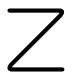
\includegraphics[keepaspectratio]{images/part001_bd86b8f3.jpg}}

In other words, when I is not bounded, if one denotes by \(\mathcal{I}\) the vector space formed by the regulated functions \(\mathbf{f}\) on I, with values in E, and admitting an integral over I, then the map \(\mathbf{f} \mapsto \int_{\mathrm{I}} \mathbf{f}(t) dt\) is not continuous when one endows \(\mathcal{I}\) with the topology of uniform convergence on I (cf.~II, p.~53, cor. 2).

We shall seek sufficient conditions to assure the validity of prop. 1, under the following hypotheses:

\(1^{\circ}\) I is an arbitrary interval in \(\mathbf{R}\) , the function \(\mathbf{f}_{\alpha}\) is regulated on I, and admits an integral over I;

\(2^{\circ}\) the family \((\mathbf{f}_{\alpha})\) converges uniformly to \(\mathbf{f}\) with respect to the filter \(\mathfrak{F}\) on every compact interval contained in I.

Writing \(\mathfrak{K}(\mathrm{I})\) for the directed set of compact intervals contained in I (II, p.~64), the left-hand side of formula (1) of II, p.~68 can be written as \(\lim_{\mathfrak{F}}\left(\lim_{\mathrm{J}\in \mathfrak{K}(\mathrm{I})}\int_{\mathrm{J}}\mathbf{f}_{\alpha}(t)dt\right)\) ; on
the other hand, taking account of prop. 1 (II, p.~68), and also the fact that the family \((\mathbf{f}_{\alpha})\) is uniformly convergent on every compact interval \(J \subset I\) , the right-hand side of (1) (II, p.~68) can be written as \(\lim_{\mathrm{J} \in \mathfrak{K}(\mathrm{I})} \left( \lim_{\mathfrak{F}} \int_{\mathrm{J}} \mathbf{f}_{\alpha}(t) dt \right)\) . One thus sees that prop. 1 of
II, p.~19 extends when one can interchange the limits of the map(J, \(\alpha\) ) \(\mapsto \int_{J} f_{\alpha}(t) dt\) with respect to the filter F and with respect to the filter \(\Phi\) of sections of the directed set K(I). Now, we know a sufficient condition for this interchange to be justified, namely the existence of the limit of the map (J, \(\alpha\) ) \(\mapsto \int_{J} f_{\alpha}(t) dt\) with respect to the product filter \(\Phi \times F\) (Gen.~Top., I, p.~81, cor. to th. 1). We shall transform this condition into an equivalent, more manageable, condition.

In the first place, since E is complete, in order that \((\mathbf{J}, \alpha) \mapsto \int_{\mathbf{J}} \mathbf{f}_{\alpha}(t) dt\) should have a limit with respect to \(\Phi \times F\) it is necessary and sufficient that, for every \(\varepsilon > 0\) , there should exist a compact interval \(J_{0} \subset I\) and a set \(M \in F\) such that, for any elements \(\alpha\) , \(\beta\) of M and compact interval \(J \supset J_{0}\) contained in I, one has

\[
\left\| \int_ {J _ {0}} \mathbf {f} _ {\alpha} (t) d t - \int_ {J} \mathbf {f} _ {\beta} (t) d t \right\| \leqslant \varepsilon .\tag{4}
\]

We shall show on the other hand that this condition is itself equivalent to the following condition: for every \(\varepsilon > 0\) there exists a compact interval \(J_0 \subset I\) and a set \(M \in \mathfrak{F}\) such that, for any \(\alpha\) of \(M\) and any compact interval \(J \supset J_0\) contained in \(I\) , one has

\[
\left\| \int_ {J _ {0}} \mathbf {f} _ {\alpha} (t) d t - \int_ {J} \mathbf {f} _ {\alpha} (t) d t \right\| \leqslant \varepsilon .\tag{5}
\]

It is indeed clear that this last condition is necessary; conversely, if it is satisfied, there exists (by the uniform convergence of \((\mathbf{f}_{\alpha})\) on every compact interval) a set \(N \in F\) such that, for any \(\alpha\) , \(\beta\) in N one has

\[
\left\| \int_ {\mathrm{J} _ {0}} \mathbf {f} _ {\alpha} (t) d t - \int_ {\mathrm{J} _ {0}} \mathbf {f} _ {\beta} (t) d t \right\| \leqslant \varepsilon ;\tag{6}
\]

and therefore \(\left\|\int_{J_{0}}\mathbf{f}_{\alpha}(t)dt-\int_{J}\mathbf{f}_{\beta}(t)dt\right\|\leqslant2\varepsilon\) for any \(\alpha\) and \(\beta\) in \(M\cap N\in\mathfrak{F}\) and for any compact interval \(J\supset J_{0}\) .

Finally, the lemma of II, p.~65 allows us to put this last condition in the following equivalent form: for every \(\varepsilon > 0\) there exist a compact interval \(\mathbf{J}_0 \subset \mathbf{I}\) and a set \(\mathbf{M} \in \mathfrak{F}\) (depending on \(\varepsilon\) ) such that, for every compact interval \(\mathbf{K} \subset \mathbf{I}\) having no interior point in common with \(\mathbf{J}_0\) , and every \(\alpha \in \mathbf{M}\) , one has \(\left\| \int_{\mathbf{K}} \mathbf{f}_{\alpha}(t) dt \right\| \leqslant \varepsilon\) .

Most often, one uses a more restrictive condition obtained by supposing that, in the last statement, the set M does not depend on \(\varepsilon\) :

DEFINITION 1. One says that the integral \(\int_{\mathrm{I}} \mathbf{f}_{\alpha}(t) dt\) is uniformly convergent for \(\alpha \in \mathrm{A}\) (or uniformly convergent over \(\mathrm{A}\) ) if, for every \(\varepsilon > 0\) there exists a compact interval \(\mathrm{J}_0 \subset J\) such that, for every compact interval \(\mathrm{K} \subset \mathrm{I}\) with no interior point in common with \(\mathrm{J}_0\) , and every \(\alpha \in \mathrm{A}\) , one has

\[
\left\| \int_ {K} \mathbf {f} _ {\alpha} (t) d t \right\| \leqslant \varepsilon .\tag{7}
\]

This definition is equivalent to saying that the family of maps \(\alpha\mapsto\int_{J}\mathbf{f}_{\alpha}(t)dt\) is uniformly convergent on A (towards the map \(\alpha\mapsto\int_{I}\mathbf{f}_{\alpha}(t)dt\) ) with respect to the filter of sections \(\Phi\) of \(\Re(I)\) ; each of the integrals \(\int_{I}\mathbf{f}_{\alpha}(t)dt\) is a fortiori convergent (the converse being false); Further, from what we have just seen (or from Gen.~Top., X, p.~281, cor. 2):

PROPOSITION 3. Let \((\mathbf{f}_{\alpha})\) be a family of regulated functions on an interval I such that: \(1^{\circ}\) with respect to the filter \(\mathfrak{F}\) the family \((\mathbf{f}_{\alpha})\) converges uniformly to a function \(\mathbf{f}\) (regulated on I) on every compact interval contained in I; \(2^{\circ}\) the integral \(\int_{I} \mathbf{f}_{\alpha}(t) dt\) is uniformly convergent for every \(\alpha \in A\) . Under these hypotheses the integral \(\int_{I} \mathbf{f}(t) dt\) is convergent, and one has

\[
\lim _ {\mathfrak {F}} \int_ {\mathrm{I}} \mathbf {f} _ {\alpha} (t) d t = \int_ {\mathrm{I}} \mathbf {f} (t) d t.\tag{8}
\]

The hypotheses of prop. 3 are fulfilled when for example I is a bounded interval, the \(\mathbf{f}_{\alpha}\) are uniformly bounded on I, and converge uniformly to \(\mathbf{f}\) on every compact interval contained in I; indeed, if \(\| \mathbf{f}_{\alpha}(x)\| \leqslant h\) for all \(x\in \mathrm{I}\) and all \(\alpha\) , and if \(\mathrm{J}_0\) is such that the difference between the lengths of I and \(\mathrm{J}_0\) is \(\leqslant \varepsilon /h\) , then condition (7) is satisfied for every interval \(\mathrm{K}\subset \mathrm{I}\) with no interior point in common with \(\mathrm{J}_0\) .

As with prop. 1 of II, p.~68, two corollaries to prop. 3 are important in applications:

COROLLARY 1. Let \((\mathbf{f}_{n})\) be a sequence of regulated functions on an arbitrary interval I, converging uniformly to a function f on each compact interval contained in I; if the integral \(\int_{I} \mathbf{f}_{n}(t) dt\) is uniformly convergent, then the integral \(\int_{I} \mathbf{f}(t) dt\) is convergent, and

\[
\lim _ {n \to \infty} \int_ {\mathrm{I}} \mathbf {f} _ {n} (t) d t = \int_ {\mathrm{I}} \mathbf {f} (t) d t.\tag{9}
\]

Remark. The hypotheses imposed in this corollary are sufficient, but not necessary, for the validity of formula (9); we shall generalize this formula later, at the same time as the concept of integral (see INT, IV), and obtain much less restrictive conditions.

COROLLARY 2. Let A be a subset of a topological space F, and f a map of I × A into a complete normed space E over R, such that, for every \(\alpha \in A\) , the function \(x \mapsto \mathbf{f}(x, \alpha)\) is regulated on I. If, on the one hand, the functions \(x \mapsto \mathbf{f}(x, \alpha)\) converge uniformly on every compact interval contained in I to a function \(x \mapsto \mathbf{f}(x)\) as \(\alpha\) tends to \(\alpha_{0} \in \overline{A}\) while remaining in A; if, on the other hand, the integral \(\int_{I} \mathbf{f}(x, \alpha) dx\) is uniformly convergent on A, then the integral \(\int_{I} \mathbf{f}(x) dx\) is convergent, and one has

\[
\lim _ {\alpha \rightarrow \alpha_ {0}, \alpha \in A} \int_ {I} \mathbf {f} (x, \alpha) d x = \int_ {I} \mathbf {f} (x) d x.\tag{10}
\]

In particular:

PROPOSITION 4 (``continuity of an improper integral with respect to a parameter''). Let F be a compact space, let I be any interval in R, and f a continuous map from I × F into a complete normed space E over R; if the integral \(\mathbf{h}(\alpha) = \int_{\mathrm{I}} \mathbf{f}(x, \alpha) dx\) is uniformly convergent on F, it is a continuous function of \(\alpha\) on F.

In view of prop. 2 of II, p.~69, this proposition also follows from the continuity of a uniform limit of continuous functions (Gen.~Top., X, p.~282, th. 2).

\subsection{NORMALLY CONVERGENT INTEGRALS}

Let \((\mathbf{f}_{\alpha})_{\alpha\in\mathrm{A}}\) be a family of regulated functions on an arbitrary interval \(I\subset R\) , with values in a complete normed space E over R. Suppose that there exists a finite real regulated function g on I such that, for every \(x\in I\) and every \(\alpha\in A\) , \(\|f_{\alpha}(x)\|\leqslant g(x)\) and also the integral \(\int_{I}g(t)dt\) is convergent. Under these conditions the integral \(\int_{I}\mathbf{f}_{\alpha}(t)dt\) is absolutely and uniformly convergent on A; in fact, for every compact interval K contained in I,

\[
\left\| \int_ {K} \mathbf {f} _ {\alpha} (t) d t \right\| \leqslant \int_ {K} g (t) d t
\]

and the convergence of the integral \(\int_{I} g(t) dt\) implies that for every \(\varepsilon > 0\) there exists a compact interval \(J \subset I\) such that for every compact interval \(K \subset I\) disjoint from J one has \(\int_{K} g(t) dt \leqslant \varepsilon\) . When there exists a real function g having the preceding properties one says that the integral \(\int_{I} f_{\alpha}(t) dt\) is normally convergent on A (cf.~Gen.~Top., X, p.~296).

An integral can be uniformly convergent on A without being normally convergent. *This happens for the sequence \((f_n)\) of real functions defined by the conditions \(f_n(x) = 1 / x\) for \(n \leqslant x \leqslant n + 1\) , and \(f_n(x) = 0\) for the other values of \(x\) in \(\mathbf{I} = [\mathbf{0}, +\infty[\) . It is immediate that the integral \(\int_{1}^{\infty} f_n(t) dt\) is uniformly convergent, but not normally convergent, since the relation \(g(x) \geqslant f_n(x)\) for each \(x \in \mathbf{I}\) and all \(n\) entails that \(g(x) \geqslant 1 / x\) , and consequently that the integral of \(g\) over \(\mathbf{I}\) is not convergent.*

In particular, let us consider a series whose general term \(u_{n}\) is a regulated function on an interval I, and suppose that the series with general term \(\|u_{n}(x)\|\) (which is a regulated function on I) converges uniformly on every compact interval contained in I, and such that the series with general term \(\int_{I}\|\mathbf{u}_{n}(t)\|dt\) is convergent; then (II, p.~66, prop. 2) the (regulated) function \(g(x)\) , the sum of the series with general term \(\|u_{n}(x)\|\) , is such that the integral \(\int_{I}g(t)dt\) is convergent. If one puts \(f_{n}=\sum_{p=1}^{n}u_{p}\) , then the integral \(\int_{I}f_{n}(t)dt\) is normally convergent, for one has

\[
\left\| \mathbf {f} _ {n} (x) \right\| \leqslant \sum_ {p = 1} ^ {n} \left\| \mathbf {u} _ {p} (x) \right\| \leqslant g (x)
\]

for all \(x \in \mathrm{I}\) and all \(n\) ; in consequence, the sum \(\mathbf{f}\) of the series with general term \(\mathbf{u}_n\) is a regulated function on \(\mathrm{I}\) such that the integral \(\int_{\mathrm{I}} \mathbf{f}(t) dt\) is convergent, and one has

\[
\int_ {\mathrm{I}} \mathbf {f} (t) d t = \sum_ {n = 1} ^ {\infty} \int_ {\mathrm{I}} \mathbf {u} _ {n} (t) d t\tag{11}
\]

(``term-by-term integration of a series on a non-compact interval'').

\subsection{DERIVATIVE WITH RESPECT TO A PARAMETER OF AN INTEGRAL OVER A COMPACT INTERVAL}

Let A be a compact neighbourhood of a point \(\alpha_{0}\) in the field R (resp. the field C), let I = {[}a, b{]} be a compact interval in R, and f a continuous map of I × A into a complete normed space E over R (resp. C). We have seen (II, p.~69, prop. 2) that under these conditions \(\mathbf{g}(\alpha) = \int_{a}^{b} \mathbf{f}(t, \alpha) dt\) is a continuous function on A. Let us seek sufficient conditions for g to admit a derivative at the point \(\alpha_{0}\) . One has, for \(\alpha \neq \alpha_{0}\) ,

\[
\frac {\mathbf {g} (\alpha) - \mathbf {g} (\alpha_ {0})}{\alpha - \alpha_ {0}} = \int_ {a} ^ {b} \frac {\mathbf {f} (t , \alpha) - \mathbf {f} (t , \alpha_ {0})}{\alpha - \alpha_ {0}} d t
\]

so (II, p.~69, cor. 2), if the functions \(x \mapsto \frac{\mathbf{f}(x, \alpha) - \mathbf{f}(x, \alpha_0)}{\alpha - \alpha_0}\) converge uniformly on I to a (necessarily continuous) function \(x \mapsto \mathbf{h}(x)\) as \(\alpha\) tends to \(\alpha_0\) (while remaining \(\neq \alpha_0\) ), then \(\mathbf{g}\) admits a derivative equal to \(\int_{a}^{b} \mathbf{h}(t) dt\) at the point \(\alpha_0\) ; moreover, for each \(x \in I\) , \(\frac{\mathbf{f}(x, \alpha) - \mathbf{f}(x, \alpha_0)}{\alpha - \alpha_0}\) tends to \(\mathbf{h}(x)\) , so \(\mathbf{h}(x)\) is the derivative at the point \(\alpha_0\) of the map \(\alpha \mapsto \mathbf{f}(x, \alpha)\) ; we denote this derivative (called the partial derivative of \(\mathbf{f}\) with respect to \(\alpha\) ) by the notation \(\mathbf{f}_{\alpha}'(x, \alpha_0)\) ; the hypotheses we have made imply that

\[
\mathbf {g} ^ {\prime} (\alpha_ {0}) = \int_ {a} ^ {b} \mathbf {f} _ {\alpha} ^ {\prime} (t, \alpha_ {0}) d t.\tag{12}
\]

The following proposition gives a very simple sufficient condition for the validity of formula (12):

PROPOSITION 5. Suppose that the partial derivative \(\mathbf{f}_{\alpha}^{\prime}(x,\alpha)\) exists for all \(x\in \mathrm{I}\) and all \(\alpha\) in an open neighbourhood \(\mathbf{V}\) of \(\alpha_0\) , and that, for all \(\alpha \in \mathbf{V}\) , the map \(x\mapsto \mathbf{f}_{\alpha}^{\prime}(x,\alpha)\) is regulated on \(\mathrm{I}\) . Under these conditions, if \(x\mapsto \mathbf{f}_{\alpha}^{\prime}(x,\alpha)\) converges uniformly on \(\mathrm{I}\) to \(x\mapsto \mathbf{f}_{\alpha}^{\prime}(x,\alpha_0)\) as \(\alpha\) tends to \(\alpha_0\) , then the function \(\mathbf{g}(\alpha) = \int_{a}^{b}\mathbf{f}(t,\alpha)dt\) admits a derivative, given by the formula (12), at the point \(\alpha_0\) .

Indeed, for every \(\varepsilon > 0\) there exists by hypothesis an \(r > 0\) such that \(|\alpha - \alpha_0| \leqslant r\) implies \(\left\| \mathbf{f}_{\alpha}'(x, \alpha) - \mathbf{f}_{\alpha}'(x, \alpha_0) \right\| \leqslant \varepsilon\) for any \(x \in I\) . By props. 3 and 5 of I, p.~17 one has, for \(|\alpha - \alpha_0| \leqslant r\) ( \(\alpha \neq \alpha_0\) ) and for all \(x \in I\)

\[
\left| \left| \frac {\mathbf {f} (x , \alpha) - \mathbf {f} (x , \alpha_ {0})}{\alpha - \alpha_ {0}} - \mathbf {f} _ {\alpha} ^ {\prime} (x, \alpha_ {0}) \right| \right| \leqslant \varepsilon
\]

which proves the uniform convergence of \(\frac{\mathbf{f}(x,\alpha)-\mathbf{f}(x,\alpha_{0})}{\alpha-\alpha_{0}}\) to \(\mathbf{f}_{\alpha}^{\prime}(x,\alpha_{0})\) on I as \(\alpha\) tends to \(\alpha_{0}\) (remaining \(\neq\alpha_{0}\) ), and so establishes formula (12).

COROLLARY. If the partial derivative \(\mathbf{f}_{\alpha}^{\prime}(x,\alpha)\) exists on I × V and is a continuous function of \((x,\alpha)\) on this set, then the function g admits a derivative given by the formula (12) at the point \(\alpha_{0}\) .

Indeed, if W is a compact neighbourhood of \(\alpha_{0}\) contained in V, then the map \((x,\alpha)\mapsto\mathbf{f}_{\alpha}^{\prime}(x,\alpha)\) is uniformly continuous on the compact set I × W, so \(\mathbf{f}_{\alpha}^{\prime}(x,\alpha)\) tends to \(\mathbf{f}_{\alpha}^{\prime}(x,\alpha_{0})\) uniformly on I as \(\alpha\) tends to \(\alpha_{0}\) .

From prop. 5 one deduces a more general proposition which allows one to evaluate the derivative of an integral when, not only the integrand f, but also the limits of integration, depend on a parameter \(\alpha\) :

PROPOSITION 6. Supposing that the hypotheses of prop. 5 are satisfied, let \(a(\alpha)\) , \(b(\alpha)\) be two functions defined on V, with values in I; if the derivatives \(a'(\alpha_0)\) , \(b'(\alpha_0)\) exist and are finite then the function \(\mathbf{g}(\alpha) = \int_{a(\alpha)}^{b(\alpha)} \mathbf{f}(t, \alpha) dt\) admits at \(\alpha_0\) a derivative given by the formula

\[
\mathbf {g} ^ {\prime} (\alpha_ {0}) = \int_ {a (\alpha_ {0})} ^ {b (\alpha_ {0})} \mathbf {f} _ {\alpha} ^ {\prime} (t, \alpha_ {0}) d t + b ^ {\prime} (\alpha_ {0}) \mathbf {f} (b (\alpha_ {0}), \alpha_ {0}) - a ^ {\prime} (\alpha_ {0}) \mathbf {f} (a (\alpha_ {0}), \alpha_ {0}).\tag{13}
\]

Indeed, for all \(\alpha \in \mathbf{V}\) distinct from \(\alpha_0\) one can write

\[
\begin{array}{c} \frac {\mathbf {g} (\alpha) - \mathbf {g} (\alpha_ {0})}{\alpha - \alpha_ {0}} = \int_ {a (\alpha_ {0})} ^ {b (\alpha_ {0})} \frac {\mathbf {f} (t , \alpha) - \mathbf {f} (t , \alpha_ {0})}{\alpha - \alpha_ {0}} d t + \frac {1}{\alpha - \alpha_ {0}} \int_ {b (\alpha_ {0})} ^ {b (\alpha)} \mathbf {f} (t, \alpha) d t \\ - \frac {1}{\alpha - \alpha_ {0}} \int_ {a (\alpha_ {0})} ^ {a (\alpha)} \mathbf {f} (t, \alpha) d t. \end{array}
\]

By prop. 5 of II, p.~74, the first integral on the right-hand side tends to \(\int_{a(\alpha_0)}^{b(\alpha_0)} \mathbf{f}'_\alpha(t, \alpha_0) dt\) as \(\alpha\) tends to \(\alpha_0\) . In the second integral we replace \(\mathbf{f}(t, \alpha)\) by \(\mathbf{f}(b(\alpha_0), \alpha_0)\) and show that the difference tends to 0. We put \(\mathbf{M} = \operatorname{Max}\big( \| \mathbf{f}(b(\alpha_0), \alpha_0) \|, |b'(\alpha_0)| + 1 \big)\) ; the function \(b(\alpha)\) being continuous at the point \(\alpha_0\) and the function \(\mathbf{f}\) continuous at the point \((b(\alpha_0), \alpha_0)\) , for every \(\varepsilon\) such that \(0 < \varepsilon < 1\) there exists an \(r > 0\) such that the relation \(|\alpha - \alpha_0| \leqslant r\) entails that \(\| \mathbf{f}(t, \alpha) - \mathbf{f}(b(\alpha_0), \alpha_0) \| \leqslant \varepsilon\) for all \(t\) belonging to the interval with endpoints \(b(\alpha_0)\) and \(b(\alpha)\) ; thus one may also suppose that the relation \(|\alpha - \alpha_0| \leqslant r\) entails \(\left| \frac{b(\alpha) - b(\alpha_0)}{\alpha - \alpha_0} - b'(\alpha_0) \right| \leqslant \varepsilon\) .

By the mean value formula (II, p.~62, formula (17)) one thus has

\[
\left\| \frac {1}{\alpha - \alpha_ {0}} \int_ {b (\alpha_ {0})} ^ {b (\alpha)} \mathbf {f} (t, \alpha) d t - \frac {b (\alpha) - b (\alpha_ {0})}{\alpha - \alpha_ {0}} \mathbf {f} (b (\alpha_ {0}), \alpha_ {0}) \right\| \leqslant \left| \frac {b (\alpha) - b (\alpha_ {0})}{\alpha - \alpha_ {0}} \right| \varepsilon
\]

and consequently

\[
\left\| \frac {1}{\alpha - \alpha_ {0}} \int_ {b (\alpha_ {0})} ^ {b (\alpha)} \mathbf {f} (t, \alpha) d t - b ^ {\prime} (\alpha_ {0}) \mathbf {f} (b (\alpha_ {0}), \alpha_ {0}) \right\| \leqslant 2 \mathrm{M} \varepsilon
\]

which shows that \(\frac{1}{\alpha - \alpha_0} \int_{b(\alpha_0)}^{b(\alpha)} \mathbf{f}(t, \alpha) dt\) tends to \(b'(\alpha_0)\mathbf{f}(b(\alpha_0), \alpha_0)\) . In the same way one shows that \(\frac{1}{\alpha - \alpha_0} \int_{a(\alpha_0)}^{a(\alpha)} \mathbf{f}(t, \alpha) dt\) tends to \(a'(\alpha_0)\mathbf{f}(a(\alpha_0), \alpha_0)\) .

\subsection{DERIVATIVE WITH RESPECT TO A PARAMETER OF AN INTEGRAL OVER A NON-COMPACT INTERVAL}

The set V having the same meaning as in prop. 5 of II, p.~74, suppose now that I is any interval in R, and that f is a continuous map from I × V into E; if the integral \(\mathbf{g}(\alpha) = \int_{\mathrm{I}} \mathbf{f}(t, \alpha) dt\) exists for all \(\alpha \in V\) and is a continuous function of \(\alpha\) , the function g need not have a derivative equal to \(\int_{\mathrm{I}} \mathbf{f}'_{\alpha}(t, \alpha_0) dt\) at the point \(\alpha_0\) , even if \(\mathbf{f}'_{\alpha}(x, \alpha)\)

converges uniformly to \(\mathbf{f}_{\alpha}^{\prime}(x,\alpha_{0})\) on every compact interval contained in I, and if the integral \(\int_{\mathrm{I}}\mathbf{f}_{\alpha}^{\prime}(t,\alpha)dt\) exists for all \(\alpha \in \mathrm{V}\) (cf.~II, p.~87, exerc. 3).

A sufficient condition for formula (12) (II, p.~74) to remain valid is given by the following proposition:

PROPOSITION 7. Let I be an arbitrary interval in \(\mathbf{R}\) , and \(\mathbf{f}\) a continuous function on \(\mathrm{I} \times \mathrm{V}\) . Suppose that:

\(1^{\circ}\) the partial derivative \(\mathbf{f}_{\alpha}^{\prime}(x,\alpha)\) exists for all \(x\in \mathrm{I}\) and all \(\alpha \in \mathrm{V}\) , and, for all \(\alpha \in \mathrm{V}\) , the map \(x\mapsto \mathbf{f}_{\alpha}^{\prime}(x,\alpha)\) is regulated on \(\mathrm{I}\) ;

\(2^{\circ}\) for all \(\alpha \in \mathrm{V}\) , \(\mathbf{f}_{\alpha}^{\prime}(x,\beta)\) converges uniformly to \(\mathbf{f}_{\alpha}^{\prime}(x,\alpha)\) on every compact interval contained in I, as \(\beta\) tends to \(\alpha\) ;

\(3^{\circ}\) the integral \(\int_{\mathrm{I}}\mathbf{f}_{\alpha}^{\prime}(t,\alpha)dt\) is uniformly convergent on \(\mathrm{V}\) ;

\(4^{\circ}\) the integral \(\int_{\mathrm{I}}\mathbf{f}(t,\alpha_0)dt\) is convergent.

In these circumstances the integral \(\mathbf{g}(\alpha)=\int_{\mathrm{I}}\mathbf{f}(t,\alpha)dt\) is uniformly convergent on V, and the function g admits at every point of V a derivative given by the formula

\[
\mathbf {g} ^ {\prime} (\alpha) = \int_ {\mathrm{I}} \mathbf {f} _ {\alpha} ^ {\prime} (t, \alpha) d t.\tag{14}
\]

The uniform convergence of \(\int_{\mathrm{I}} \mathbf{f}_{\alpha}'(t, \alpha) dt\) on V means that the function \(\alpha \mapsto \int_{\mathrm{J}} \mathbf{f}_{\alpha}'(t, \alpha) dt\) converges uniformly on V with respect to the filter of sections \(\Phi\) of the directed set \(\Re(\mathrm{I})\) of compact intervals J contained in I. Let us put \(\mathbf{u}_{\mathrm{J}}(\alpha) = \int_{\mathrm{J}} \mathbf{f}(t, \alpha) dt\) ; the hypotheses show that on the one hand \(\mathbf{u}_{\mathrm{J}}(\alpha_0)\) has a limit with respect to \(\Phi\) , and on the other hand, by virtue of prop. 5 of II, p.~74, that \(\mathbf{u}_{\mathrm{J}}'(\alpha) = \int_{\mathrm{J}} \mathbf{f}_{\alpha}'(t, \alpha) dt\) for all \(\alpha \in \mathrm{V}\) . We can therefore apply th. 1 of II, p.~52 to the functions \(\mathbf{u}_{\mathrm{J}}\) , the rôle of the set of indices being taken here by \(\Re(\mathrm{I})\) , and that of the filter on this set by the filter \(\Phi\) ; the proposition follows immediately.

Remarks. 1) Conditions \(1^{\circ}\) and \(2^{\circ}\) of prop. 7 are satisfied a fortiori when \(\mathbf{f}_{\alpha}^{\prime}(x,\alpha)\) is a continuous function of \((x,\alpha)\) on \(\mathrm{I} \times \mathrm{V}\) .

\begin{enumerate}
\def\labelenumi{\arabic{enumi})}
\setcounter{enumi}{1}
\tightlist
\item
  When, in an integral \(\int_{a(\alpha)}^{b(\alpha)}\mathbf{f}(t,\alpha)dt\) , the endpoints of the interval are finite functions of the parameter, the study of this integral as a function of \(\alpha\) can be related to that of an integral over {[}0, 1{]}; indeed, by the change of variable \(t = a(\alpha)(1 - u) + b(\alpha)u\) , one has
\end{enumerate}

\[
\int_ {a (\alpha)} ^ {b (\alpha)} \mathbf {f} (t, \alpha) d t = \int_ {0} ^ {1} \mathbf {f} (a (\alpha) (1 - u) + b (\alpha) u, \alpha) (b (\alpha) - a (\alpha)) d u.
\]

\subsection{CHANGE OF ORDER OF INTEGRATION}

Let \(I = [a, b]\) and \(A = [c, d]\) be two compact intervals in \(R\) ; let \(f\) be a continuous function on \(I \times A\) with values in a complete normed space \(E\) over \(R\) ; by prop. 2 of II, p.~69, \(\int_{a}^{b} f(x, \alpha) dx\) is a continuous function of \(\alpha\) on \(A\) ; its integral \(\int_{c}^{d} \left( \int_{a}^{b} f(x, \alpha) dx \right) d\alpha\) is also denoted, for simplicity, by \(\int_{c}^{d} d\alpha \int_{a}^{b} f(x, \alpha) dx\) .

PROPOSITION 8. If \(\mathbf{f}\) is continuous on \(\mathrm{I} \times \mathrm{A}\) one has

\[
\int_ {c} ^ {d} d \alpha \int_ {a} ^ {b} \mathbf {f} (x, \alpha) d x = \int_ {a} ^ {b} d x \int_ {c} ^ {d} \mathbf {f} (x, \alpha) d \alpha\tag{15}
\]

(``formula for interchanging the order of integration'').

We shall show that, for all \(y \in A\) , one has

\[
\int_ {c} ^ {y} d \alpha \int_ {a} ^ {b} \mathbf {f} (x, \alpha) d x = \int_ {a} ^ {b} d x \int_ {c} ^ {y} \mathbf {f} (x, \alpha) d \alpha .\tag{16}
\]

Since the two sides of (16) are functions of \(y\) , and equal for \(y = c\) , it will suffice to prove that they are differentiable on \(]c\) , \(d[\) and that their derivatives are equal at every point of this interval. If one puts \(\mathbf{g}(\alpha) = \int_{a}^{b} \mathbf{f}(x, \alpha) dx\) , and \(\mathbf{h}(x, y) = \int_{c}^{y} \mathbf{f}(x, \alpha) dx\) , the relation (16) can be written

\[
\int_ {c} ^ {y} \mathbf {g} (\alpha) d \alpha = \int_ {a} ^ {b} \mathbf {h} (x, y) d x.
\]

Now, the derivative of the first term with respect to \(y\) is \(\mathbf{g}(y)\) , while that of the second is \(\int_{a}^{b} \mathbf{h}_{y}'(x, y) dx\) , by II, p.74, corollary, since \(\mathbf{h}_{y}'(x, y) = \mathbf{f}(x, y)\) is continuous on \(I \times A\) ; the two expressions thus obtained are identical.

Suppose now that A = {[}c, d{]} is a compact interval in R, and I an arbitrary interval in R; let f be a continuous function on I × A, with values in E, such that the integral \(\mathbf{g}(\alpha) = \int_{\mathrm{I}} \mathbf{f}(t, \alpha) dt\) is convergent for all \(\alpha \in A\) ; even if \(\mathbf{g}(\alpha)\) is continuous on A one cannot always interchange the order of integration in the integral \(\int_{c}^{d} d\alpha \int_{I} \mathbf{f}(t, \alpha) dt\) , for the integral \(\int_{I} dt \int_{c}^{d} \mathbf{f}(t, \alpha) d\alpha\) may not exist, or it may be different from the integral \(\int_{c}^{d} d\alpha \int_{I} \mathbf{f}(t, \alpha) dt\) (cf.~II, p.~87, exerc. 7). One has, however, the following result:

PROPOSITION 9. If the function \(\mathbf{f}\) is continuous on \(\mathrm{I} \times \mathrm{A}\) , and if the integral \(\int_{\mathrm{I}} \mathbf{f}(t, \alpha) dt\) is uniformly convergent on \(\mathrm{A}\) , then the integral \(\int_{\mathrm{I}} dt \int_{c}^{d} \mathbf{f}(t, \alpha) d\alpha\) is convergent, and one has

\[
\int_ {c} ^ {d} d \alpha \int_ {\mathrm{I}} \mathbf {f} (t, \alpha) d t = \int_ {\mathrm{I}} d t \int_ {c} ^ {d} \mathbf {f} (t, \alpha) d \alpha .\tag{17}
\]

For every compact interval J contained in I, put \(\mathbf{u}_{\mathrm{J}}(\alpha) = \int_{\mathrm{J}} \mathbf{f}(t, \alpha) dt\) . The hypothesis entails that with respect to the filter of sections \(\Phi\) of the directed set \(\Re(\mathrm{I})\) the continuous function \(u_{J}\) converges uniformly on A to \(\int_{I} f(t, \alpha) dt\) ; thus (II, p.~68, prop. 1), \(\int_{c}^{d} d\alpha \int_{J} f(t, \alpha) dt\) has limit \(\int_{c}^{d} d\alpha \int_{I} f(t, \alpha) dt\) with respect to \(\Phi\) ; but, by prop. 8 (II, p.~77), one has

\[
\int_ {c} ^ {d} d \alpha \int_ {\mathrm{J}} \mathbf {f} (t, \alpha) d t = \int_ {\mathrm{J}} d t \int_ {c} ^ {d} \mathbf {f} (t, \alpha) d \alpha .\tag{18}
\]

The preceding result thus means that the integral \(\int_{I} dt \int_{c}^{d} \mathbf{f}(t, \alpha) d\alpha\) is convergent, and on passing to the limit with respect to \(\Phi\) in the relation (18), one obtains (17).

\setcounter{exercisegroup}{0}
\refstepcounter{exercisegroup}
\section*{Exercises on \S\arabic{exercisegroup}}
\phantomsection
\addcontentsline{toc}{section}{Exercises on \protect\S\arabic{exercisegroup}}

\begin{enumerate}
\def\labelenumi{\arabic{enumi})}
\tightlist
\item
  Let \((f_{\alpha})\) be a set of real functions, defined on an interval \(\mathrm{I} \subset \mathbf{R}\) , each admitting a strict primitive on \(\mathrm{I}\) , and forming a directed set for the relation \(\leqslant\) . Let \(f\) be the upper envelope of the family \((f_{\alpha})\) ; suppose that \(f\) admits a strict primitive on \(\mathrm{I}\) . Show that if \(g_{\alpha}\) (resp. \(g\) ) is the primitive of \(f_{\alpha}\) (resp. \(f\) ) which vanishes at a point \(x_0 \in \mathrm{I}\) , then \(g\) is the upper envelope of the family \((g_{\alpha})\) on the intersection \(\mathrm{I} \cap [x_0, +\infty[\) and its lower envelope on the intersection \(\mathrm{I} \cap ] - \infty\) , \(x_0]\) . (Restricting to the first of these intervals, show that if \(u\) is the upper envelope of \((g_{\alpha})\) on \(\mathrm{I} \cap [x_0, +\infty[\) then one has \(u(x + h) - u(x) \leqslant g(x + h) - g(x)\) for \(h > 0\) ; then prove that, for all \(\alpha\) , one has \(u(x + h) - u(x) \geqslant g_{\alpha}(x + h) - g_{\alpha}(x)\) , and conclude from this last inequality that \(\liminf_{h \to 0} (u(x + h) - u(x))/h \geqslant f(x)\) ; deduce the proposition from this.)
\end{enumerate}

Give an example of an increasing sequence \((f_n)\) of continuous functions on an interval I which are uniformly bounded, but whose upper envelope does not admit a strict primitive on I.

\begin{enumerate}
\def\labelenumi{\arabic{enumi})}
\setcounter{enumi}{1}
\item
  Show that for a function \(\mathbf{f}\) to be a step function on an interval I it is necessary and sufficient that it have only a finite number of points of discontinuity, and be constant on every interval where it is continuous.
\item
  Let \(\mathbf{f}\) be a regulated function on an interval \(I \subset \mathbf{R}\) , taking its values in a complete normed space \(E\) over \(\mathbf{R}\) ; show that for every compact subset \(H\) of \(I\) the set \(\mathbf{f}(H)\) is relatively compact in \(E\) ; give an example where \(\mathbf{f}(H)\) is not closed in \(E\) .
\item
  Give an example of a continuous real function \(f\) on a compact interval \(\mathrm{I} \subset \mathbf{R}\) , such that the composite function \(x \mapsto \operatorname{sgn}(f(x))\) is not regulated on \(\mathrm{I}\) (even though \(\operatorname{sgn}\) is regulated on \(\mathbf{R}\) ).
\item
  Let \(\mathbf{f}\) be a vector function defined on a compact interval \(\mathrm{I} = [a, b] \subset \mathbf{R}\) , taking its values in a complete normed space \(\mathrm{E}\) ; one says that \(\mathbf{f}\) is of bounded variation on \(\mathrm{I}\) if there exists a number \(m > 0\) such that, for every finite strictly increasing sequence \((x_i)_{0 \leqslant i \leqslant n}\) of
\end{enumerate}

points of I such that \(x_0 = a\) and \(x_n = b\) , one has \(\sum_{i=0}^{n-1} \| \mathbf{f}(x_{i+1}) - \mathbf{f}(x_i) \| \leqslant m\) .

\begin{enumerate}
\def\labelenumi{\alph{enumi})}
\item
  Show that \(\mathbf{f}(\mathrm{I})\) is relatively compact in E (argue by contradiction).
\item
  Show that \(\mathbf{f}\) is regulated on I (prove that when \(x\) tends to a point \(x_0 \in \mathrm{I}\) , remaining \(>x_0\) , the function \(\mathbf{f}\) cannot have two different cluster points, and use \(a\) )).
\end{enumerate}

\begin{enumerate}
\def\labelenumi{\arabic{enumi})}
\setcounter{enumi}{5}
\tightlist
\item
  For a function \(\mathbf{f}\) , with values in a complete normed space \(E\) , and defined on an open interval \(I \subset R\) , to be equal to a regulated function on \(I\) at all points of the complement of a countable subset of \(I\) , it is necessary and sufficient that it satisfy the following condition: for every \(x \in I\) and every \(\varepsilon > 0\) there exist a number \(h > 0\) and two elements \(a\) , \(b\) of \(E\) such that one has \(\| \mathbf{f}(y) - a \| \leqslant \varepsilon\) for every \(y \in [x, x + h]\) , except for at most a countably infinite number of points of this interval, and \(\| \mathbf{f}(z) - b \| \leqslant \varepsilon\) for all \(z \in [x - h, x]\) except for at most a countably infinite number of points of this interval.
\end{enumerate}

* 7) Show that the function equal to \(\sin(1/x)\) for \(x \neq 0\) and to 0 for \(x = 0\) , admits a strict primitive on \(\mathbf{R}\) (remark that \(x^2 \sin(1/x)\) admits a derivative at every point).

Deduce from this that if \(g(x,u,v)\) is a polynomial in u, v, its coefficients being continuous functions of x on an interval I containing 0, then the function equal to \(g(x,\sin1/x,\cos1/x)\) for \(x\neq0\) , and to a suitable value \(\alpha\) (to be determined) for x=0, admits a strict primitive on I; give an example where \(\alpha\neq g(0,0,0)\) .

* 8) Show that there exists a continuous function on \([-1, +1]\) admitting a finite derivative at every point of this interval, this derivative being equal to \(\sin\left(\frac{1}{\sin 1/x}\right)\) at points \(x\) different from \(1/n\pi\) ( \(n\) an integer \(\neq 0\) ) and from 0. (On a neighbourhood of \(x = 1/n\pi\) make the change of variable \(x = \frac{1}{n\pi + \operatorname{Arc} \sin u}\) and use exerc. 7; by means of the same change of variable, show that there exists a constant \(a > 0\) independent of \(n\) such that

\[
\left| \int_ {2 / (2 n + 1) \pi} ^ {2 / (2 n - 1) \pi} \sin \left(\frac {1}{\sin \frac {1}{x}}\right) d x \right| \leqslant \frac {a}{n ^ {3}};
\]

and deduce that if one puts

\[
g (x) = \lim _ {\varepsilon \rightarrow 0} \int_ {\varepsilon} ^ {x} \sin \left(\frac {1}{\sin \frac {1}{t}}\right) d t,
\]

then g has a derivative equal to 0 at the point x = 0.) *

\begin{enumerate}
\def\labelenumi{\arabic{enumi})}
\setcounter{enumi}{8}
\item
  Let \(\mathbf{f}\) be a regulated function on a compact interval \(\mathrm{I} = [a, b]\) . Show that for every \(\varepsilon > 0\) there exists a continuous function \(\mathbf{g}\) on \(\mathrm{I}\) such that \(\int_{a}^{b} \| \mathbf{f}(t) - \mathbf{g}(t) \| dt \leqslant \varepsilon\) (reduce to the case where \(\mathbf{f}\) is a step function). Deduce that there exists a polynomial \(\mathbf{h}\) (with coefficients in E) such that \(\int_{a}^{b} \| \mathbf{f}(t) - \mathbf{h}(t) \| dt \leqslant \varepsilon\) .
\item
  Let \(\mathbf{f}\) be a regulated function on \([a, b]\) , taking values in E, let \(\mathbf{g}\) be a regulated function on \([a, c]\) ( \(c > b\) ), taking its values in F, and let \((\mathbf{x}, \mathbf{y}) \mapsto [\mathbf{x}, \mathbf{y}]\) be a continuous bilinear map from \(\mathrm{E} \times \mathrm{F}\) into G (E, F, G being complete normed spaces). Show that
\end{enumerate}

\[
\lim _ {h \rightarrow 0, h > 0} \int_ {a} ^ {b} [ \mathbf {f} (t). \mathbf {g} (t + h) ] d t = \int_ {a} ^ {b} [ \mathbf {f} (t). \mathbf {g} (t) ] d t
\]

(reduce to the case where \(\mathbf{f}\) is a step function).

\begin{enumerate}
\def\labelenumi{\arabic{enumi})}
\setcounter{enumi}{10}
\tightlist
\item
  With the same hypotheses as in exerc. 10 show that for every \(\varepsilon > 0\) there exists a number \(\rho > 0\) such that for every subdivision of \([a, b]\) into intervals \([x_i, x_{i+1}]\) of length \(\leqslant \rho\) ( \(0 \leqslant i \leqslant n-1\) ) one has
\end{enumerate}

\[
\left\| \int_ {a} ^ {b} [ \mathbf {f} (t). \mathbf {g} (t) ] d t - \sum_ {i = 0} ^ {n - 1} [ \mathbf {f} (u _ {i}). \mathbf {g} (v _ {i}) ] (x _ {i + 1} - x _ {i}) \right\| \leqslant \varepsilon
\]

for any choice, for each index i, of points \(u_{i}\) , \(v_{i}\) in \([x_{i}, x_{i+1}]\) (reduce to the case where f and g are step functions).

¶ 12) One says that a sequence \((x_{n})\) of real numbers in the interval \([0, 1]\) is uniformly distributed in this interval if

\[
\lim _ {n \to \infty} \frac {\nu_ {n} (\alpha , \beta)}{n} = \beta - \alpha\tag{1}
\]

for every pair of numbers \(\alpha\) , \(\beta\) such that \(0 \leqslant \alpha \leqslant \beta \leqslant 1\) , where \(\nu_{n}(\alpha, \beta)\) denotes the number of indices \(i\) such that \(1 \leqslant i \leqslant n\) and \(\alpha \leqslant x_{i} \leqslant \beta\) .

Show that if the sequence \((x_{n})\) is uniformly distributed and if \(\mathbf{f}\) is a regulated function on \([0, 1]\) , one has

\[
\lim _ {n \rightarrow \infty} \frac {1}{n} \sum_ {i = 1} ^ {n} \mathbf {f} (x _ {i}) = \int_ {0} ^ {1} \mathbf {f} (t) d t\tag{2}
\]

(reduce to the case where \(\mathbf{f}\) is a step function). Converse.

Show that for the sequence \((x_{n})\) to be uniformly distributed it is enough that the relation (2) should hold for every real function f belonging to a dense set in the space of real continuous functions on {[}0, 1{]} endowed with the topology of uniform convergence.

¶ 13) Let \(f\) be a real regulated function on a compact interval \([a, b]\) . Put

\[
r (n) = \frac {b - a}{n} \sum_ {k = 1} ^ {n} f \left(a + k \frac {b - a}{n}\right) - \int_ {a} ^ {b} f (t) d t.
\]

\begin{enumerate}
\def\labelenumi{\alph{enumi})}
\tightlist
\item
  Show that if \(f\) is increasing on \([a, b]\) one has
\end{enumerate}

\[
0 \leqslant r (n) \leqslant \frac {b - a}{n} \Bigl (f (b) - f (a) \Bigr).
\]

\begin{enumerate}
\def\labelenumi{\alph{enumi})}
\setcounter{enumi}{1}
\tightlist
\item
  If \(f\) is continuous and admits a regulated bounded right derivative on \([a, b[\) , show that one has \(\lim_{n\to \infty}nr(n) = \frac{b - a}{2} (f(b) - f(a))\) (putting \(x_{k} = a + k\frac{b - a}{n}\) ), remark that one has
\end{enumerate}

\[
r (n) = \sum_ {k = 0} ^ {n - 1} \int_ {x _ {k}} ^ {x _ {k + 1}} \left(f (x _ {k + 1}) - f (t)\right) d t,
\]

and apply prop. 5 of II, p.~57).

\begin{enumerate}
\def\labelenumi{\alph{enumi})}
\setcounter{enumi}{2}
\tightlist
\item
  Give an example of a function \(f\) , increasing and continuous on \([a, b]\) , such that \(nr(n)\) does not tend to \(\frac{b - a}{2} (f(b) - f(a))\) as \(n\) grows indefinitely {[}take for \(f\) the limit of a decreasing sequence \((f_n)\) of increasing functions whose graphs are broken lines such that
\end{enumerate}

\[
f _ {n} \left(a + k \frac {b - a}{2 ^ {n}}\right) = f \left(a + k \frac {b - a}{2 ^ {n}}\right) \quad \text { for } \quad 0 \leqslant k \leqslant 2 ^ {n}
\]

and

\[
(b - a) \sum_ {k = 1} ^ {2 ^ {n}} f _ {n} \left(a + k \frac {b - a}{2 ^ {n}}\right) - 2 ^ {n} \int_ {a} ^ {b} f _ {n} (t) d t \geqslant \frac {3}{4} (b - a) \left(f _ {n} (b) - f _ {n} (a)\right) \Biggr ].
\]

\begin{enumerate}
\def\labelenumi{\arabic{enumi})}
\setcounter{enumi}{13}
\tightlist
\item
  Let \(\mathbf{f}\) be a vector function which is the primitive of a regulated function \(\mathbf{f}'\) on \([a, b]\) , and such that \(\mathbf{f}(a) = \mathbf{f}(b) = 0\) . Show that if \(\mathbf{M}\) is the least upper bound of \(\| \mathbf{f}'(x)\|\) over the set of points of \([a, b]\) where \(\mathbf{f}'\) is continuous, then
\end{enumerate}

\[
\left\| \int_ {a} ^ {b} \mathbf {f} (t) d t \right\| \leqslant \mathrm{M} \frac {(b - a) ^ {2}}{4}.
\]

\begin{enumerate}
\def\labelenumi{\arabic{enumi})}
\setcounter{enumi}{14}
\tightlist
\item
  Let \(\mathbf{f}\) be a continuous real function, strictly increasing on an interval \([0, a]\) , and such that \(f(0) = 0\) ; let \(g\) be its inverse function, defined and strictly increasing on \([0, f(a)]\) ; show that
\end{enumerate}

\[
x y \leqslant \int_ {0} ^ {x} f (t) d t + \int_ {0} ^ {y} g (u) d u
\]

for \(0 \leqslant x \leqslant a\) and \(0 \leqslant y \leqslant f(a)\) , equality occurring only if \(y = f(x)\) (study the variation of \(xy - \int_{0}^{x} f(t) dt\) ) as a function of x (y remaining fixed). Deduce that for \(x \geqslant 0\) , \(y \geqslant 0\) , p \textgreater{} 1, \(p' = p/(p - 1)\) , one has \(xy \leqslant ax^{p} + by^{p'}\) for a \textgreater{} 0, b \textgreater{} 0 and \((pa)^{p'}(p'b)^{p} \geqslant 1\) .

\begin{enumerate}
\def\labelenumi{\arabic{enumi})}
\setcounter{enumi}{15}
\tightlist
\item
  Let \(\mathbf{f}\) be a regulated vector function on \(\mathrm{I} = [a, b] \subset \mathbf{R}\) , let \(\mathbf{u}\) be a primitive of \(\mathbf{f}\) on \(\mathrm{I}\) and \(\mathrm{D}\) a closed convex set containing \(\mathbf{u}(\mathrm{I})\) . Show that if \(g\) is a real monotone function on \(\mathrm{I}\) one has
\end{enumerate}

\[
\int_ {a} ^ {b} \mathbf {f} (t) g (t) d t = (\mathbf {u} (b) - \mathbf {c}) g (b) + (\mathbf {c} - \mathbf {u} (a)) g (a)
\]

where \(\mathbf{c}\) belongs to D (reduce to the case where \(g\) is a monotone step function). Deduce that if \(f\) is a real regulated function on I then there exists a \(c \in \mathrm{I}\) such that

\[
\int_ {a} ^ {b} f (t) g (t) d t = g (a) \int_ {a} ^ {c} f (t) d t + g (b) \int_ {c} ^ {b} f (t) d t
\]

(``the second mean value theorem'').

\begin{enumerate}
\def\labelenumi{\arabic{enumi})}
\setcounter{enumi}{16}
\tightlist
\item
  Let \(g\) be a real function admitting a continuous derivative, and \(\neq 0\) on \([a, x]\) ; if \(f\) is a real function having a regulated \((n + 1)^{th}\) derivative on \([a, x]\) , show that the remainder \(r_n(x)\) in the Taylor expansion of order \(n\) for \(f\) at the point \(a\) can be written
\end{enumerate}

\[
r _ {n} (x) = (g (x) - g (a)) \frac {(x - \xi) ^ {n}}{n !} \frac {f ^ {(n + 1)} (\xi)}{g ^ {\prime} (\xi)}
\]

where \(a < \xi < x\) (use the integral form for \(r_{n}(x)\) ).

\begin{enumerate}
\def\labelenumi{\arabic{enumi})}
\setcounter{enumi}{17}
\tightlist
\item
  Let \(f\) be a finite real function, continuous on an open interval \(I\) . For \(f\) to be convex on \(I\) it is necessary and sufficient that for every \(x \in I\) one has
\end{enumerate}

\[
\operatorname * {l i m s u p} _ {h \to \infty} \left(\frac {1}{2 h} \int_ {x - h} ^ {x + h} f (t) d t - f (x)\right) \geqslant 0
\]

(argue as in exerc. 9 of I, p.~46).

\begin{enumerate}
\def\labelenumi{\arabic{enumi})}
\setcounter{enumi}{18}
\tightlist
\item
  Let \(f\) be a convex function on an interval \(I\) , let \(h\) be a number \(> 0\) , and \(I_h\) the intersection of \(I\) and the intervals \(I + h\) and \(I - h\) ; show that, if \(I_h\) is not empty, the function
\end{enumerate}

\[
g _ {h} (x) = \frac {1}{2 h} \int_ {x - h} ^ {x + h} f (t) d t
\]

is convex on \(\mathrm{I}_h\) ; if \(h < k\) one has \(g_h \leqslant g_k\) . When \(h\) tends to 0 show that \(g_h\) tends uniformly to \(f\) on every compact interval contained in the interior of \(\mathrm{I}\) .

\begin{enumerate}
\def\labelenumi{\arabic{enumi})}
\setcounter{enumi}{19}
\tightlist
\item
  Show that as \(n\) increases indefinitely the polynomial
\end{enumerate}

\[
f _ {n} (x) = \frac {\int_ {0} ^ {x} (1 - t ^ {2}) ^ {n} d t}{\int_ {0} ^ {1} (1 - t ^ {2}) ^ {n} d t}
\]

tends uniformly to -1 on every interval \([-1, -\varepsilon]\) , and tends uniformly to +1 on every interval \([\varepsilon, +1]\) , where \(\varepsilon > 0\) (note that \(\int_{0}^{1}(1-t^{2})^{n}dt \geqslant \int_{0}^{1}(1-t)^{n}dt\) ). Deduce that the polynomial \(g_{n}(x) = \int_{0}^{x} f_{n}(t)dt\) tends uniformly to \(|x|\) on \([-1, +1]\) , which provides a new proof of the Weierstrass theorem (Gen.~Top., X, p.~313, prop. 3).

\begin{enumerate}
\def\labelenumi{\arabic{enumi})}
\setcounter{enumi}{20}
\tightlist
\item
  Let f be a real increasing convex continuous function on an interval \([0, a]\) , and such that \(f(0) = 0\) . If \(a_{1} \geqslant a_{2} \geqslant \cdots \geqslant a_{n} \geqslant 0\) is a finite decreasing sequence of points in \([0, a]\) , show that one has
\end{enumerate}

\[
f \left(a _ {1}\right) - f \left(a _ {2}\right) + \dots + (- 1) ^ {n - 1} f \left(a _ {n}\right) \geqslant f \left(a _ {1} - a _ {2} + \dots + (- 1) ^ {n - 1} a _ {n}\right).
\]

(One can restrict oneself to the case where \(n = 2m\) is even; remark that for \(1 \leqslant j \leqslant m\) one has

\[
\int_ {\alpha} ^ {\beta} f ^ {\prime} (t) d t \leqslant \int_ {a _ {2 j}} ^ {a _ {2 j - 1}} f ^ {\prime} (t) d t
\]

where \(\alpha = a_{2j+1} - a_{2j+2} + \cdots + a_{2m-1} - a_{2m}\) and \(\beta = \alpha + (a_{2j-1} - a_{2j})\) .

\begin{enumerate}
\def\labelenumi{\arabic{enumi})}
\setcounter{enumi}{21}
\tightlist
\item
  Let f be a continuous increasing real function and \(\geqslant 0\) on the interval {[}0, 1{]}.
\end{enumerate}

\begin{enumerate}
\def\labelenumi{\alph{enumi})}
\item
  Show that there exists a convex function \(g \geqslant 0\) on {[}0,1{]} such that \(g \leqslant f\) and \(\int_0^1 g(t)dt \geqslant \frac{1}{2}\int_0^1 f(t)dt\) (cf.~I, p.~48, exerc. 23).
\item
  Show that there exists a convex function \(h\) on {[}0, 1{]} such that \(h \geqslant f\) and that
\end{enumerate}

\[
\int_ {0} ^ {1} h (t) d t \leqslant 2 \int_ {0} ^ {1} f (t) d t.
\]

(For every \(a\) such that \(0 < a \leqslant 1\) , let \(f_a\) be the function equal to \(f\) for \(0 \leqslant t \leqslant a\) and to \(f(a)\) for \(a \leqslant t \leqslant 1\) ; let A be the set of \(a \in [0,1]\) for which there exists a convex function \(h_a\) on \([0,1]\) such that \(h_a \geqslant f_a\) and \(\int_0^1 h_a(t)dt \leqslant 2\int_0^1 f_a(t)dt\) . Show that the least upper bound \(b\) of A again belongs to A, using exerc. 1 of I, p.~45. Then prove that \(f_{b} = f\) , arguing by contradiction. For this, reduce to proving the following result: if \(\varphi\) is continuous and increasing on \([0, 1]\) , not constant, and such that \(\varphi(0) = 0\) , then there is a point \(c \in ]0, 1[\) such that \(\varphi(c) > 0\) and such that the linear function \(\psi\) such that \(\psi(c) = \varphi(c)\) and

\[
\psi (2 c - 1) = 0
\]

satisfies the relation \(\psi(t) \geqslant \varphi(t)\) for \(\max(0, 2c - 1) \leqslant t \leqslant c\) .

\begin{enumerate}
\def\labelenumi{\arabic{enumi})}
\setcounter{enumi}{22}
\tightlist
\item
  Let \(\mathbf{f}\) be a vector function, continuously differentiable on an interval \([a, b] \subset \mathbf{R}\) , with values in a complete normed space.
\end{enumerate}

\begin{enumerate}
\def\labelenumi{\alph{enumi})}
\tightlist
\item
  Show that for \(a \leqslant t \leqslant b\) one has
\end{enumerate}

\[
\mathbf {f} (t) = \frac {1}{b - a} \int_ {a} ^ {b} \mathbf {f} (x) d x + \int_ {a} ^ {b} \frac {x - a}{b - a} \mathbf {f} ^ {\prime} (x) d x + \int_ {t} ^ {b} \frac {x - b}{b - a} \mathbf {f} ^ {\prime} (x) d x.
\]

\begin{enumerate}
\def\labelenumi{\alph{enumi})}
\setcounter{enumi}{1}
\tightlist
\item
  Deduce the inequalities
\end{enumerate}

\[
\| \mathbf {f} (t) \| \leqslant \frac {1}{b - a} \int_ {a} ^ {b} \| \mathbf {f} (x) \| d x + \int_ {a} ^ {b} \left\| \mathbf {f} ^ {\prime} (x) \right\| d x
\]

and

\[
\left\| \mathbf {f} \left(\frac {1}{2} (a + b)\right) \right\| \leqslant \frac {1}{b - a} \int_ {a} ^ {b} \| \mathbf {f} (x) \| d x + \frac {1}{2} \int_ {a} ^ {b} \left\| \mathbf {f} ^ {\prime} (x) \right\| d x.
\]

\setcounter{exercisegroup}{1}
\refstepcounter{exercisegroup}
\section*{Exercises on \S\arabic{exercisegroup}}
\phantomsection
\addcontentsline{toc}{section}{Exercises on \protect\S\arabic{exercisegroup}}

\begin{enumerate}
\def\labelenumi{\arabic{enumi})}
\tightlist
\item
  Let \(\alpha\) and \(\beta\) be two finite real numbers such that \(\alpha < \beta\) . Show that if \(\gamma\) and \(\delta\) are two numbers such that \(\alpha < \gamma \leqslant \delta < \beta\) then there exists a real function \(f\) defined on an interval \([0, a]\) , taking only the values \(\alpha\) and \(\beta\) , such that, on all the interval \([\varepsilon, a]\) (for \(\varepsilon > 0\) ), \(f\) is a step function and that, if one puts \(g(x) = \int_0^x f(t)dt\) , one has
\end{enumerate}

\[
\liminf _ {x \to 0,   x > 0} \frac {g (x)}{x} = \gamma , \quad \text { and } \quad \limsup _ {x \to 0,   x > 0} \frac {g (x)}{x} = \delta ;\tag{*}
\]

(take for g a function whose graph is a broken line whose consecutive sides have gradients \(\alpha\) and \(\beta\) and whose peaks occur alternately on the lines \(y = \gamma x\) , \(y = \delta x\) for \(\gamma \neq \delta\) , or on the line \(y = \gamma x\) and the parabola \(y = \gamma x + x^{2}\) for \(\gamma = \delta\) ).

By the same method show that, whether \(\gamma\) and \(\delta\) are finite or not ( \(\gamma < \delta\) ), there exists a real function f defined on \([0, a]\) , such that on every interval \([\varepsilon, a]\) (for \(\varepsilon > 0\) ), f is a step function, that the integral \(g(x) = \int_{0}^{x} f(t) dt\) exists, and that one again has the relations (*).

\begin{enumerate}
\def\labelenumi{\arabic{enumi})}
\setcounter{enumi}{1}
\tightlist
\item
  \begin{enumerate}
  \def\labelenumii{\alph{enumii})}
  \tightlist
  \item
    Let \(\mathbf{f}\) be a regulated function on an interval \([0, a]\) such that the integral \(\int_0^a \frac{\mathbf{f}(t)}{t} dt\) is convergent. Show that the integral \(\mathbf{g}(x) = \int_0^x \mathbf{f}(t) dt\) is convergent and that \(\mathbf{g}\) admits a right derivative at the point \(x = 0\) (integrate suitably by parts).
  \end{enumerate}
\end{enumerate}

\begin{enumerate}
\def\labelenumi{\alph{enumi})}
\setcounter{enumi}{1}
\tightlist
\item
  Give an example of a real function \(f\) such that the integral \(g(x) = \int_0^x f(t)dt\) is convergent and admits a right derivative at the point 0, and yet \(f(t) / t\) does not have an integral on \([0, a]\) (take for \(f(x)/x\) the derivative of a function of the form \(\cos\varphi(x)\) , where \(\varphi\) tends to \(+\infty\) as x tends to 0).
\end{enumerate}

\begin{enumerate}
\def\labelenumi{\arabic{enumi})}
\setcounter{enumi}{2}
\item
  Let \(f\) be a real function \(\geqslant 0\) , defined on an interval \(]0, a]\) and regulated on this interval, such that the integral \(g(x) = \int_0^x f(t)dt\) is convergent, but that \(g\) does not have a right derivative at the point 0. Show that there exists a function \(f_1\) , regulated on \(]0, a]\) , such that \((f_1(x))^2 = f(x)\) for all \(x\) , that the integral \(g_1(x) = \int_0^x f_1(t)dt\) converges, and that \(g_1\) has a right derivative at 0. (First consider the case where \(f\) is identical to a step function on every interval \([\varepsilon, a]\) (for \(\varepsilon > 0\) ). In this case, divide each interval on which \(f\) is constant into a large enough number of equal parts, and take \(f_1\) to be constant on each of these intervals, the sign of \(f_1\) differing on two consecutive such intervals. Proceed in the same way in the general case.)
\item
  Define on the interval \([0,1]\) two real functions f, g such that f and g admit strict primitives, but that fg is at every point of \([0,1[\) the right derivative of a continuous function which has no left derivative at a set of points having the power of the continuum (use constructions similar to those of exerc. 8 of I, p.~38 and exerc. 3 above).
\item
  \begin{enumerate}
  \def\labelenumii{\alph{enumii})}
  \tightlist
  \item
    Let \(\mathbf{f}\) be a regulated function on a bounded open interval \(]a\) , \(b[\) ; suppose that there exists a real function \(g\) , decreasing on \(]a\) , \(b[\) , such that \(\| \mathbf{f}(x) \| \leqslant g(x)\) on \(]a\) , \(b[\) and such that the integral \(\int_{a}^{b} g(t) dt\) converges. Show that if \((\varepsilon_n)\) is a sequence of numbers \(>0\) , tending to 0, and such that \(\inf_{n > 1} n \varepsilon_n > 0\) , one has
  \end{enumerate}
\end{enumerate}

\[
\lim _ {n \rightarrow + \infty} \frac {1}{n} \sum_ {k = 1} ^ {n - 1} \mathbf {f} \left(a + \varepsilon_ {n} + k \frac {b - a}{n}\right) = \int_ {a} ^ {b} \mathbf {f} (t) d t.\tag{*}
\]

\begin{enumerate}
\def\labelenumi{\alph{enumi})}
\setcounter{enumi}{1}
\item
  Give an example of a real regulated function f \textgreater{} 0 on \([0,1]\) such that the integral \(\int_{0}^{1} f(t) dt\) converges, and yet the relation (*) does not hold for \(\varepsilon_{n} = 1/n\) (take f so that its value for \(x = 2^{-p}\) is \(2^{2p}\) ).
\item
  With the same hypotheses as in a) show that
\end{enumerate}

\[
\lim _ {n \rightarrow + \infty} \frac {1}{n} \sum_ {k = 1} ^ {n} (- 1) ^ {k} \mathbf {f} \left(a + k \frac {b - a}{n}\right) = 0.
\]

\begin{enumerate}
\def\labelenumi{\arabic{enumi})}
\setcounter{enumi}{5}
\tightlist
\item
  Let \(\mathbf{f}\) be a regulated function on the interval \(]a, +\infty[\) ; suppose that there exists a real decreasing function \(g\) on \(]a, +\infty[\) such that \(\| \mathbf{f}(x)\| \leqslant g(x)\) on this interval and that the integral \(\int_{a}^{+\infty}g(t)dt\) converges. Show that the series \(\sum_{n=1}^{\infty}\mathbf{f}(a + nh)\) is absolutely convergent for every \(h > 0\) , and that
\end{enumerate}

\[
\lim _ {h \rightarrow + \infty} h \sum_ {n = 1} ^ {\infty} \mathbf {f} (a + n h) = \int_ {a} ^ {+ \infty} \mathbf {f} (t) d t.
\]

\begin{enumerate}
\def\labelenumi{\arabic{enumi})}
\setcounter{enumi}{6}
\item
  Let \(f\) and \(g\) be two regulated functions, and \(>0\) on an open interval \(]a, b[\) . Show that the integrals of the functions \(f / (1 + fg)\) and \(\inf(f, 1/g)\) over \(]a, b[\) are simultaneously either convergent or infinite.
\item
  Let \(f\) be a regulated function and \(\geqslant 0\) on an interval \([a, +\infty[\) , and let \(g\) be a differentiable increasing function defined on \([a, +\infty[\) , and such that \(g(x) - x \geqslant \lambda > 0\) for all \(x \geqslant a\) .
\end{enumerate}

Show that if one has \(f(g(x))g'(x) \leqslant kf(x)\) with k \textless{} 1 (resp. \(f(g(x))g'(x) \geqslant kf(x)\) with k \textgreater{} 1), then the integral \(\int_{a}^{+\infty} f(t) dt\) converges (resp. is equal to \(+\infty\) ) (Ermakoff's criterion: denoting the \(n^{th}\) iterate of g by \(g^n\) , consider the integral \(\int_{0}^{g^n(a)} f(t) dt\) and let n increase indefinitely).

\begin{enumerate}
\def\labelenumi{\arabic{enumi})}
\setcounter{enumi}{8}
\tightlist
\item
  Let \(\alpha\) be a number \(>0\) and \(f\) a function defined on the interval \([0, +\infty[, \geqslant 0\) and decreasing, and such that the integral \(\int_0^{+\infty} t^\alpha f(t) dt\) converges. Show that for all \(x > 0\) one has
\end{enumerate}

\[
\int_ {x} ^ {+ \infty} f (t) d t \leqslant \left(\frac {\alpha}{(\alpha + 1) x}\right) ^ {\alpha} \int_ {0} ^ {+ \infty} t ^ {\alpha} f (t) d t.
\]

(First prove this when \(f\) is constant on an interval \(]0, a]\) and zero for \(x > a\) , then for a sum of such functions, and pass to the limit for the general case.)
